\chapter{Reconstruction}
\label{chap:reconstruction}
The physics objects are detected as signals in each detector described in Section~\ref{sec:detector}.
Figure~\ref{fig:ParticlePath} shows the schematic diagram of the particles reconstructions with the ATLAS detector. 
To reconstruct the VBS process in this analysis, electrons, muons, jets, and missing transverse energy (MET) are used.
Electrons leave trajectories in the inner detector and develop an electromagnetic shower in the EM calorimeter. 
Most of the energy is absorbed in the EM calorimeter and very little energy deposit is expected in the hadron calorimeter.
Muons also leave trajectories in the inner detector.
As muons interact weakly with material, they are not absorbed in the calorimeters and leave tracks in the muon spectrometers.
Jets are spray of bundles of particles produced by the hadronization of the final-state partons, collimated towards a certain direction, which are detected as hadron shower at the EM and hadron calorimeters. While most of the particles in a jet are hadrons, it may contains leptons and photon coming from the decay products of some hadrons. Charged particles in a jet leave tracks in the inner detector and ID tracks are used to correct the observations at the calorimeter. Neutral particles. like newutirinos, are not detected at any subdetectors. but therefore they can be reconstrcted as a MET in the event.a All of these physics objets need to be effects. 
All of these physics objects need to be calibrated, in order to correct the translation from signals to original partons totake account for detector effects.
These reconstruction, identification and the calibration processes performed in the ATLAS experiment are described in this chapter.
\begin{figure}[tbp]
\begin{center}
 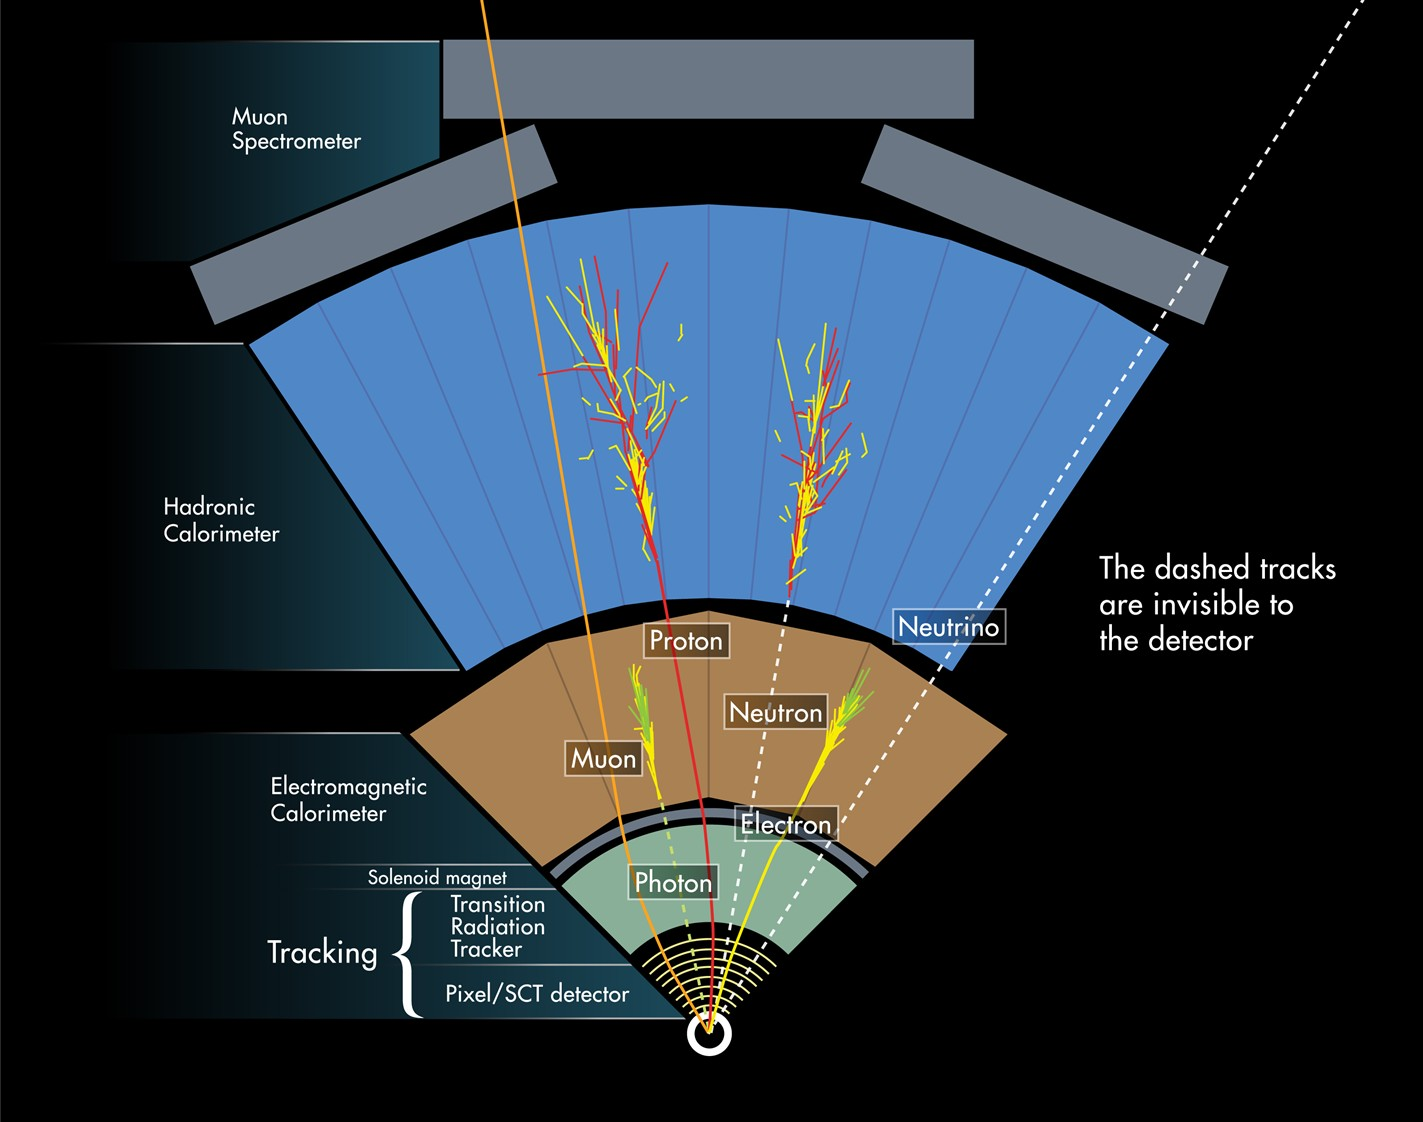
\includegraphics[width=0.80\textwidth,keepaspectratio]{figures/Reconstruction/ParticlePath}
\caption{
Schematics of the particle path
}
\label{fig:ParticlePath}
\end{center}
\end{figure}
\section{Tracks and Vertices}
The ID tracks are used for the reconstructions ofo the primary vertex and charged-particles kinematics.
The reconstruction of tracks starts from three-dimentional space points, 
reconstructed from energy deposits of charged particles, at cluster hits in the ID components. 
The track candidate is selected with a set of space points by using combinatorial Kalman filter~\cite{FRUHWIRTH1987444}. 
The best track is selected using a scoring function, then finally the track is fitted and decided. Details are described in \cite{PERF-2015-08}.
The primary vertex is reconstructed by fitting a common point to all reconstructed tracks. 
This primary vertex represents the interaction point of the proton-proton collision and is used to distinguish particles coming from the collision of interest from the ones produced by pileups.
\section{Calorimeter clusters} 
The reconstruction of the hadron and jets is based on a three-dimensional topological clustering of individual calorimeter cell signals.
The cluster formation follows cell signal-significance patterns generated by electromagnetic and hadronic showers. The clustering algorithm implicitly performs a topological noise suppression by removing cells with insignificant signals which are not in close proximity to cells with significant signals. These clusters are called Topo-clusters. Details are described in \cite{PERF-2014-07}.
\section{Electrons}
%reconstruction
Electron candidates are reconstructed from energy deposits (topo clusters)~\cite{ATL-PHYS-PUB-2017-022} in the ECal-matched to a track identified by the ID.
\begin{figure}[tbp]
\begin{center}
 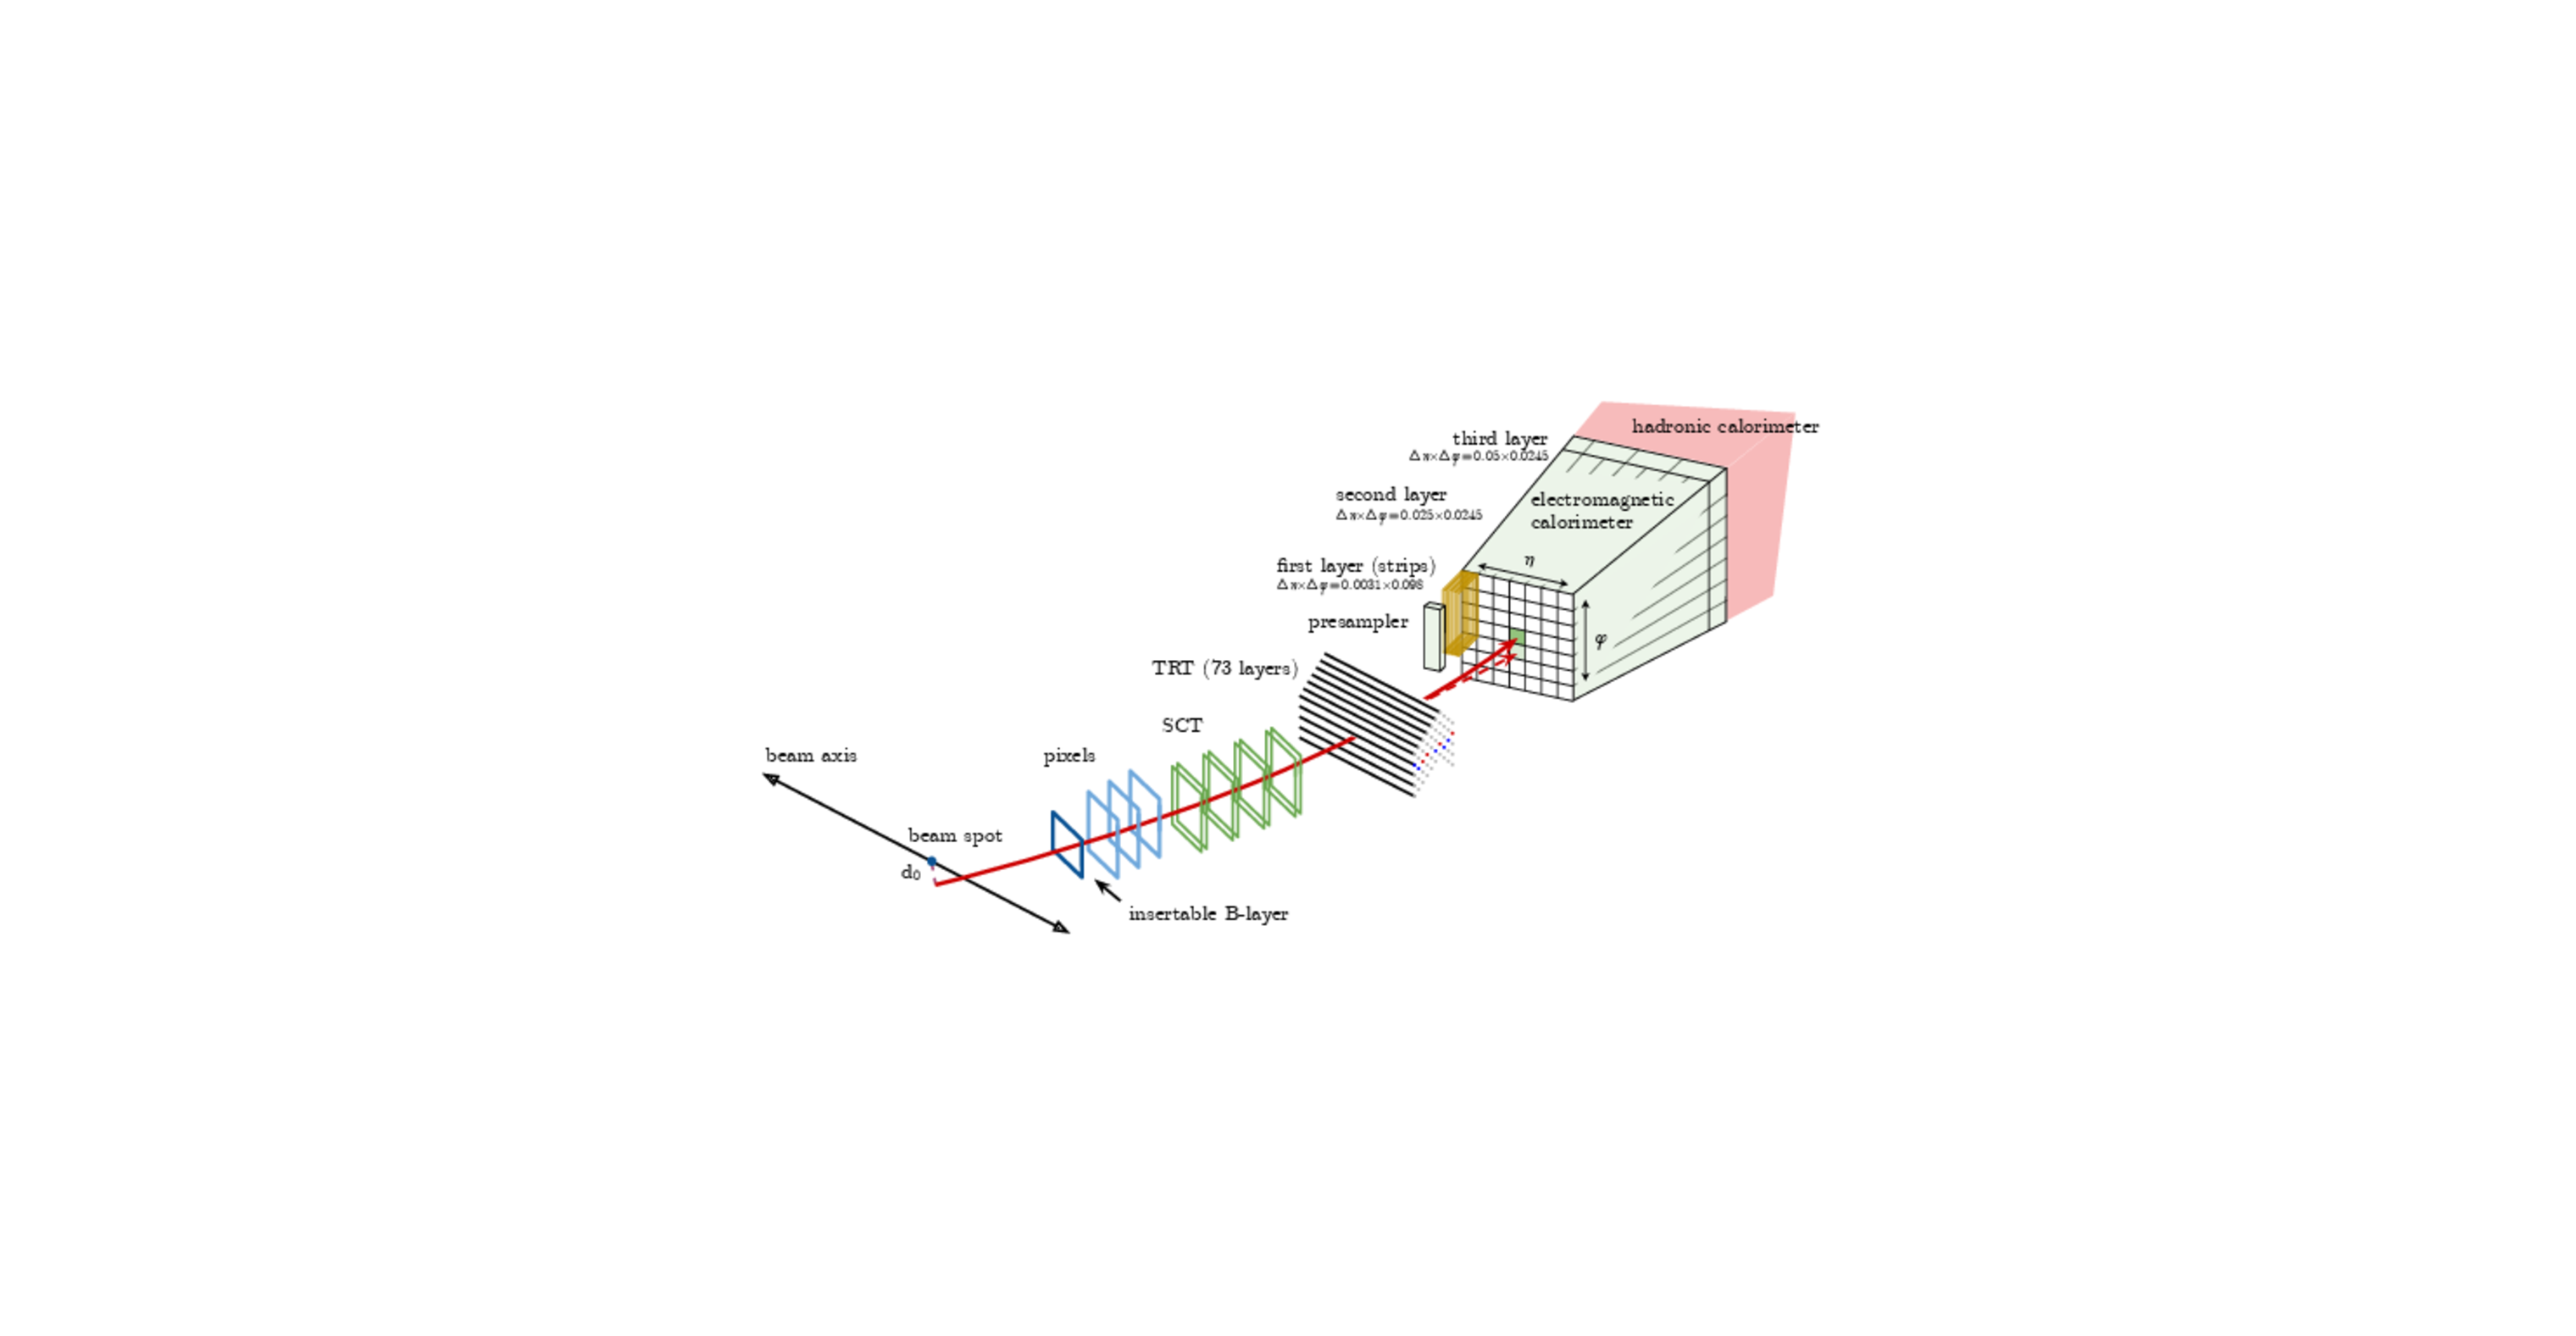
\includegraphics[width=0.80\textwidth,keepaspectratio]{figures/Reconstruction/electronPath}
\caption{
Schematics of the electron going through the detectors
}
\label{fig:electronPath}
\end{center}
\end{figure}
%identification
The reconstructed electron candidates are required to have $|\eta|<2.47$, excluding the transition region between barrel and endcap (1.37 < $|\eta|$ < 1.52).
A likelihood-based identification (LHID) is required to reduce the backgrounds from photon conversion or hadrons, e.g. charged pion and $\pi_0 \rightarrow \gamma \gamma$. 
This LHID combines various identification variables, like shower shape of the ECal and the track conditions, and the matching of the tracks and the clusters. The shower shape, or the ratio of the energy deposit in the hadronic calorimeter to that of the whole EM cluster can be used to separate the electrons from the hadrons. The track requirement is useful to distinguish the electrons from photons. Electron candidates are categorized to LooseLH, MediumLH, and TightLH corresponding to 96\%, 94\%, 88\% of identification efficiencies to signal electrons at $E_T$ = 100~GeV respectively, for the rejections of the backgrounds from misidentified hadrons, electrons from photon conversions, and non-isolated electrons originating from heavy-flavour decays. 
%In this analysis, ThightLH and Loose LH working points are employed.
%put calibration things here.....
The reconstruction and identification efficiency is measured using  $J/\Psi \rightarrow ee$ and $Z\rightarrow ee$, $Z\rightarrow ee\gamma$ events. The efficiencies are shown in Figure~\ref{fig:recoElectron}. The discrepancy between the data and the MC is corrected for using event-weight scale factors, parametrized with $E_T$ and $\eta$. Detailed information is in \cite{PERF-2017-01}.
%put momentum? resolutions here
\begin{figure}[tbp]
\begin{center}
%\subfigure[]{
 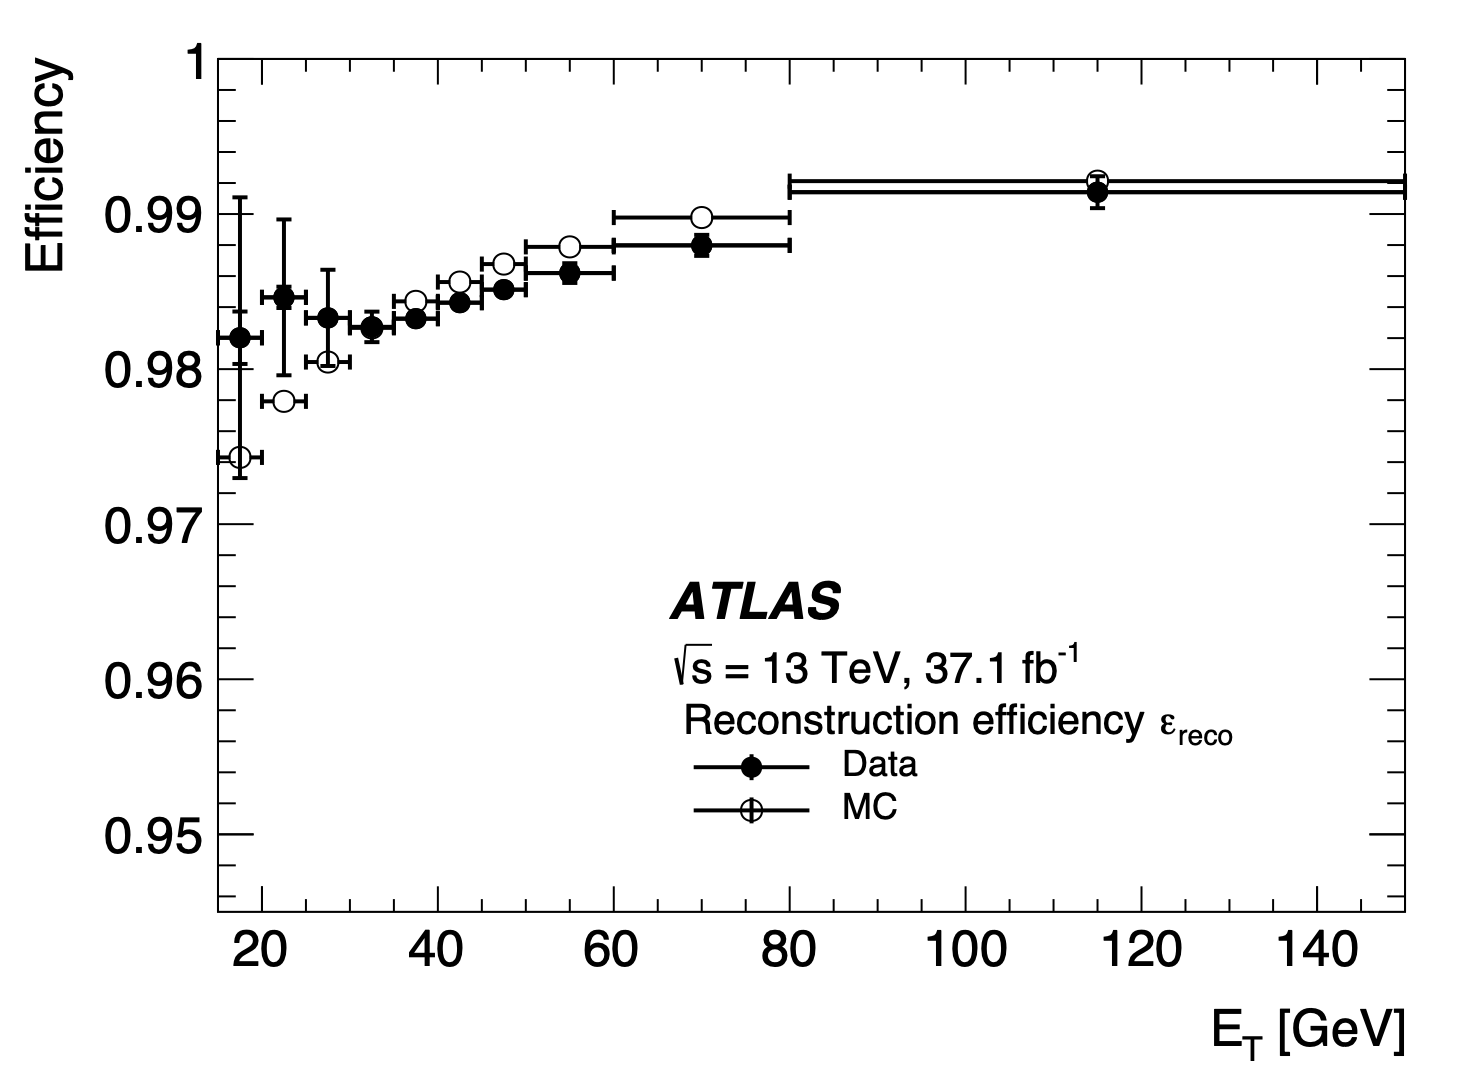
\includegraphics[width=0.50\textwidth,keepaspectratio]{figures/Reconstruction/recoElectron}
 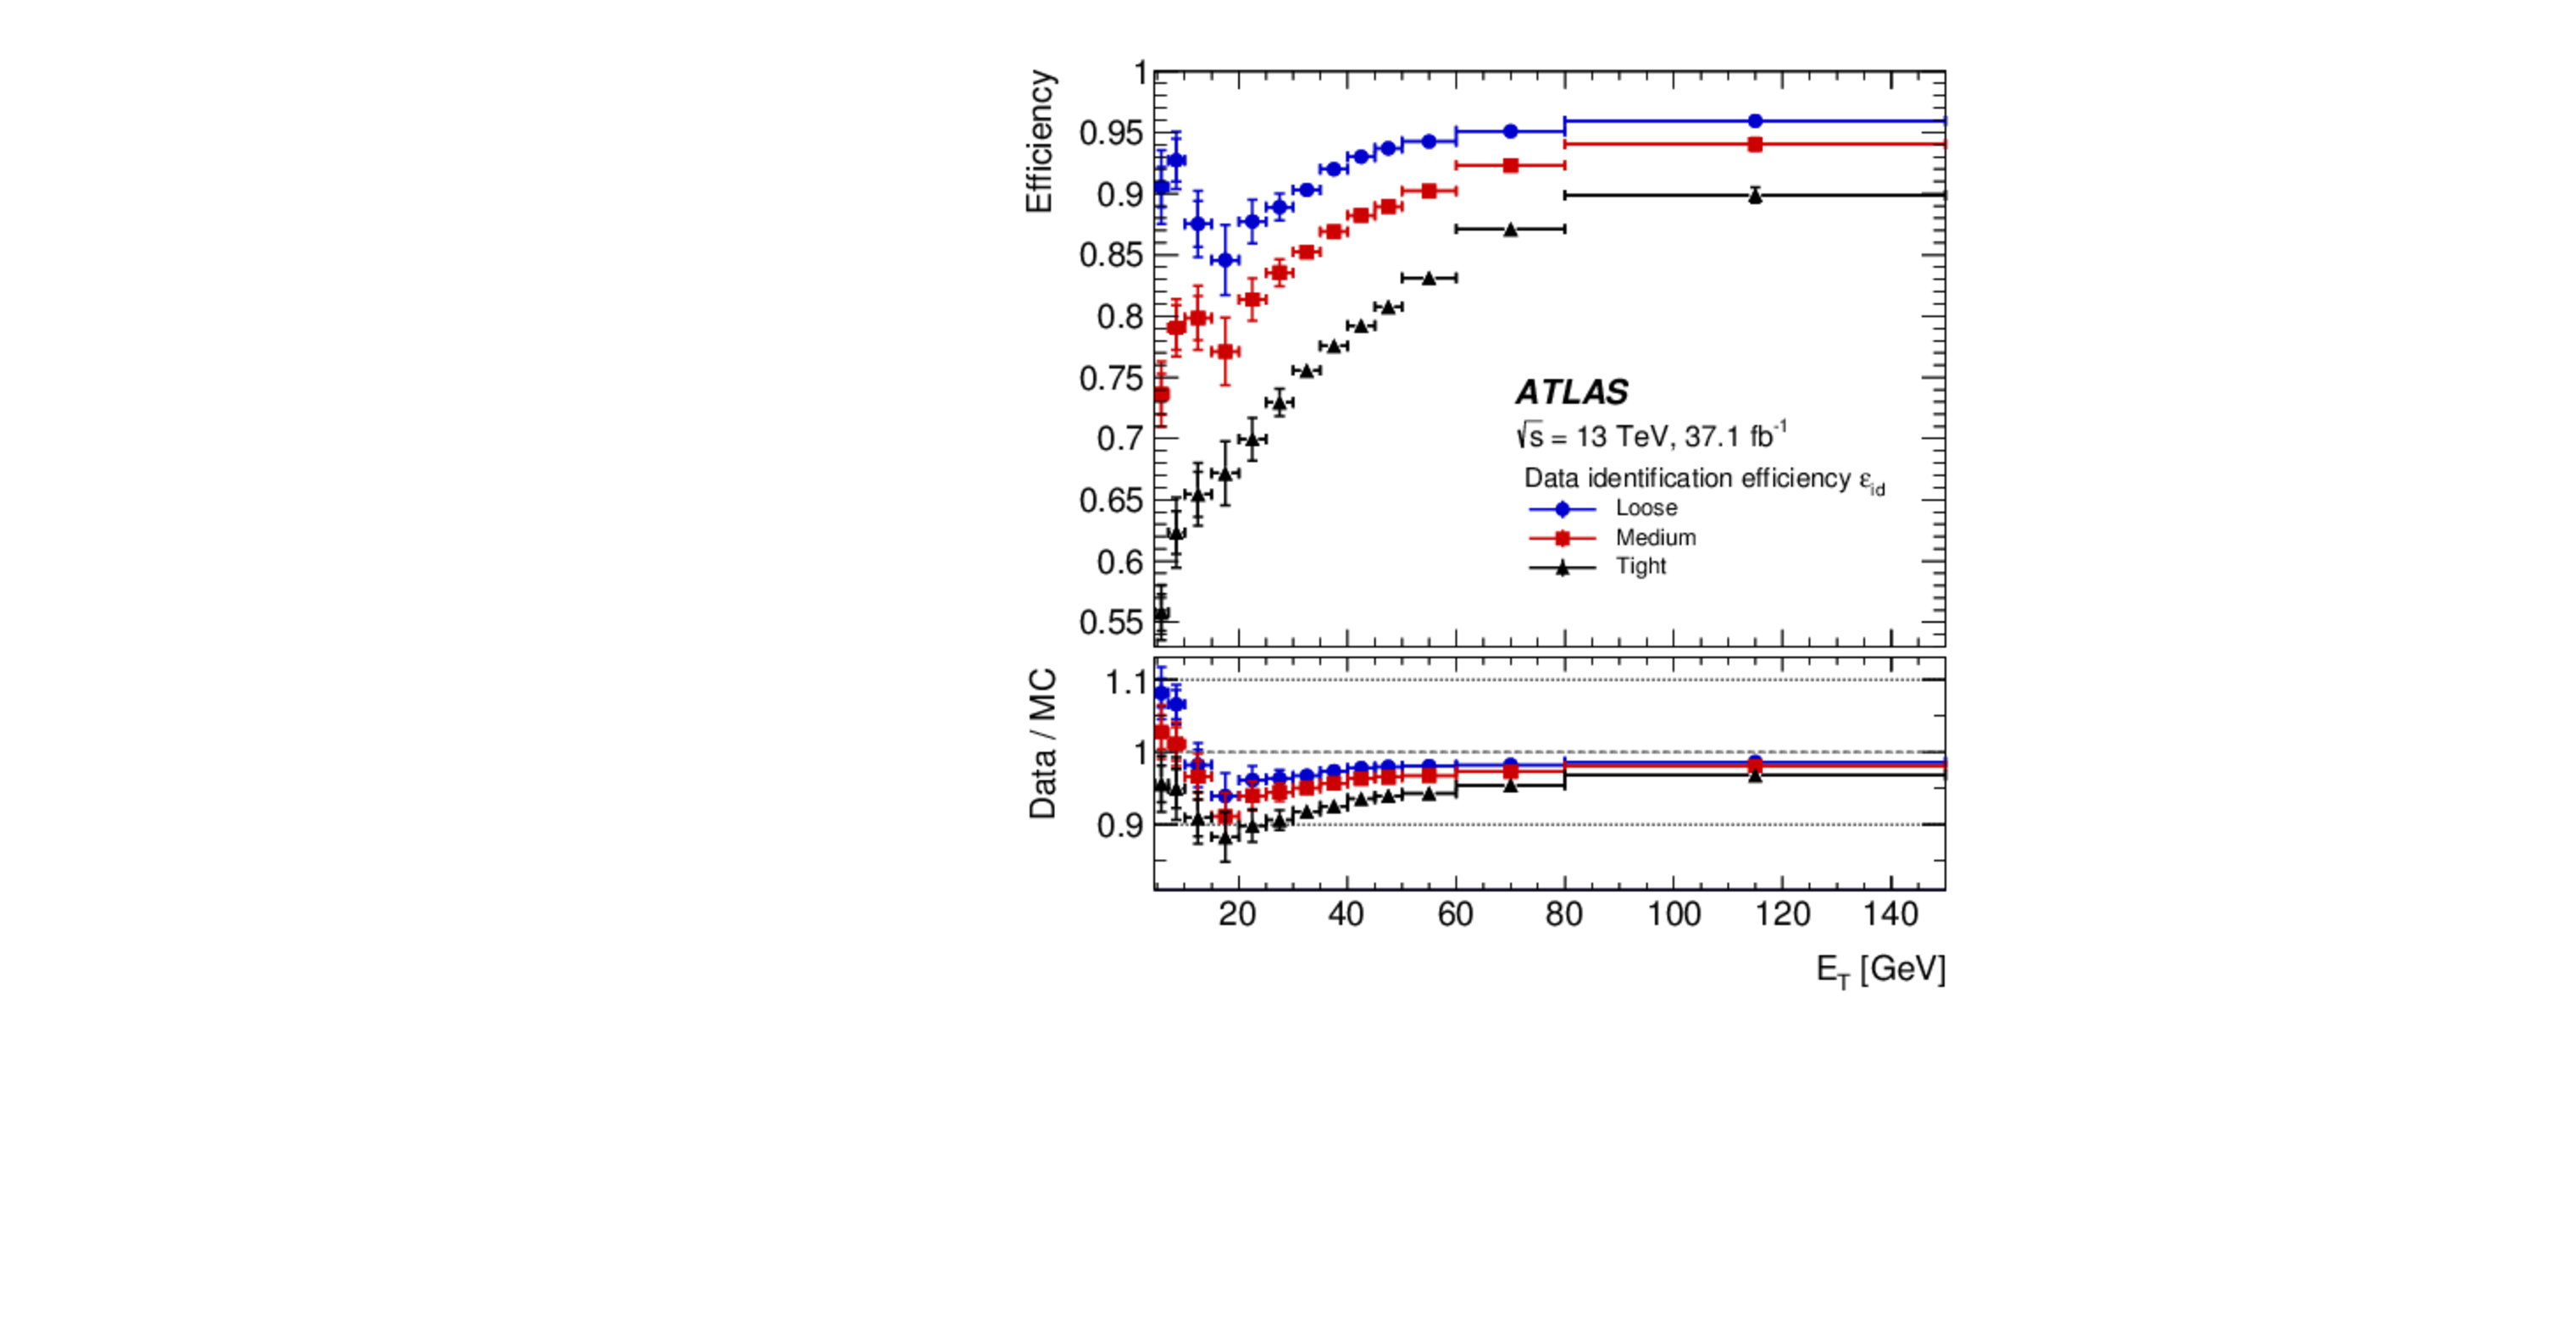
\includegraphics[width=0.45\textwidth,keepaspectratio]{figures/Reconstruction/idElectron}
%}
\caption{
electron reconstructing and identification efficiency with respect to the $E_T$
}
\label{fig:recoElectron}
\end{center}
\end{figure}
Additional requirements are applied for isolation, to reduce the contamination of jets. The two isolation working points used in this analysis, which are determined by the track and ECal informations. The selections applied in this analysis are shown in the Table~\ref{tab:electron_selection}.
Furthermore, track-to-vertex assiciation requirements are applied. 
$d_0$ is a minimum distance between the primary vertex (PV) and the track, and $\sigma_{d_0}$ is its uncertainty. $z_0$ is the tranverse impact parameter relative to the beamline.
\begin{table}[ht]
\resizebox{0.8\textwidth}{!}{
\begin{tabular}[ht]{|l|c|c|c|}
  \hline
  & \emph{Loose} & \emph{Tight}\\
  \hline
  \hline
  $p_T$ & 7~GeV & 30~GeV\\
  \hline
  $|\eta|$ & \multicolumn{2}{c|}{$|\eta| < 2.47$ \notin [1.37,1.52]} \\
  \hline
  Identification & LooseLH & TightLH \\
  \hline
  Isolation &  FCLoose $(p_T <100~GeV)$                   &  FixedCutHighPtCaloOnly \\
            &  no isolation requirement $( >100~GeV )$ & \\
  \hline
  $|d_{0}/\sigma_{d_0}|$ & \multicolumn{2}{c|}{ <~5 }\\ 
  \hline
  $| z_{0} \sin{\theta}|$ & \multicolumn{2}{c|}{ <~0.5~mm }\\
  \hline
 \end{tabular}}
 \caption{Summary of electron selection used in this analysis}
 \label{tab:electron_selection}
\end{table}
\section{Muons}
%reconstruction
Muons are reconstructed by the combination of the tracks in the Inner Detector (ID) and Muon Spectrometer (MS). 
%Figure~\ref{fig:recoMuon} shows the schematic diagram of the muon in the detectors.
%find and put the schematic of the muons
Several algorithms are used for the reconstruction: 
combined (CB) muons which require independent tracks both in ID and the MS. CB muons are of highest quality, but have least acceptance. 
Segment-tagged (ST) muons require an ID track with only one hit in the MS, which allows recovering the low-$p_T$ muons. 
Calorimeter-tagged (CT) muons are reconstructed by requiring one ID track and energy deposits in the calorimeter, whose energy agrees with the expected value for a minimum-ionizing particle. CT muons are used to increase the acceptance in the region of $|\eta| < 0.1$, corresponding to the region without the muon spectometers due to the layout of the calorimeter cables. 
%reconstruction efficiency of calibration things
The muon reconstruction efficiency is measured with samples of $J/\Psi \rightarrow \mu\mu$ and $Z\rightarrow \mu\mu$, as well as the momentum scale and resolution.
The reconstruction efficiency is found to be close to 99\% over most of the covered phase space ($|\eta|$ < 2.5 and 5 < $p_{T}$ < 100 GeV). The isolation efficiency varies between 93 and 100 \% depending on the selection applied and on the momentum of the muon. Both efficiencies are checked to be well reproduced in MC simulation. 
%In the central region of the detector, the momentum resolution is measured to be 1.7 \% (2.3 \%), and the momentum scale is known with an uncertainty of 0.05 \%. In the region $|\eta|$ > 2.2, the $p_T$ resolution for muons is 2.9 \% while the precision of the momentum scale for low-$p_T$ muons is about 0.2 \% \cite{}.
The further instructions are shown in \cite{MUON-2018-03}.
%identification
\begin{table}[ht]
\resizebox{0.8\textwidth}{!}{
\begin{tabular}[ht]{|l|c|c|c|}
  \hline
  & \emph{Loose} & \emph{Tight}\\
  \hline
  \hline
  $p_T$ & 7~GeV & 30~GeV\\
  \hline
  $|\eta|$ & \multicolumn{2}{c|}{$|\eta| < 2.5$} \\
  \hline
  Identification & Loose & Medium \\
  \hline
  Isolation &  FCLoose $(p_T <100~GeV)$                   &  FixedCutHighPtCaloOnly \\
            &  no isolation requirement $( >100~GeV )$ & \\
  \hline
  $|d_{0}/\sigma_{d_0}|$ & \multicolumn{2}{c|}{ <~3 }\\ 
  \hline
  $| z_{0} \sin{\theta}|$ & \multicolumn{2}{c|}{ <~0.5~mm }\\
  \hline
 \end{tabular}}
 \caption{Summary of muon selection used in this analysis}
 \label{tab:muon_selection}
\end{table}
Similar to the electron, the isolation requirement is also applied to the muons, as shown in the Table~\ref{tab:muon_selection}.
\begin{figure}[tbp]
\begin{center}
%\subfigure[]{
 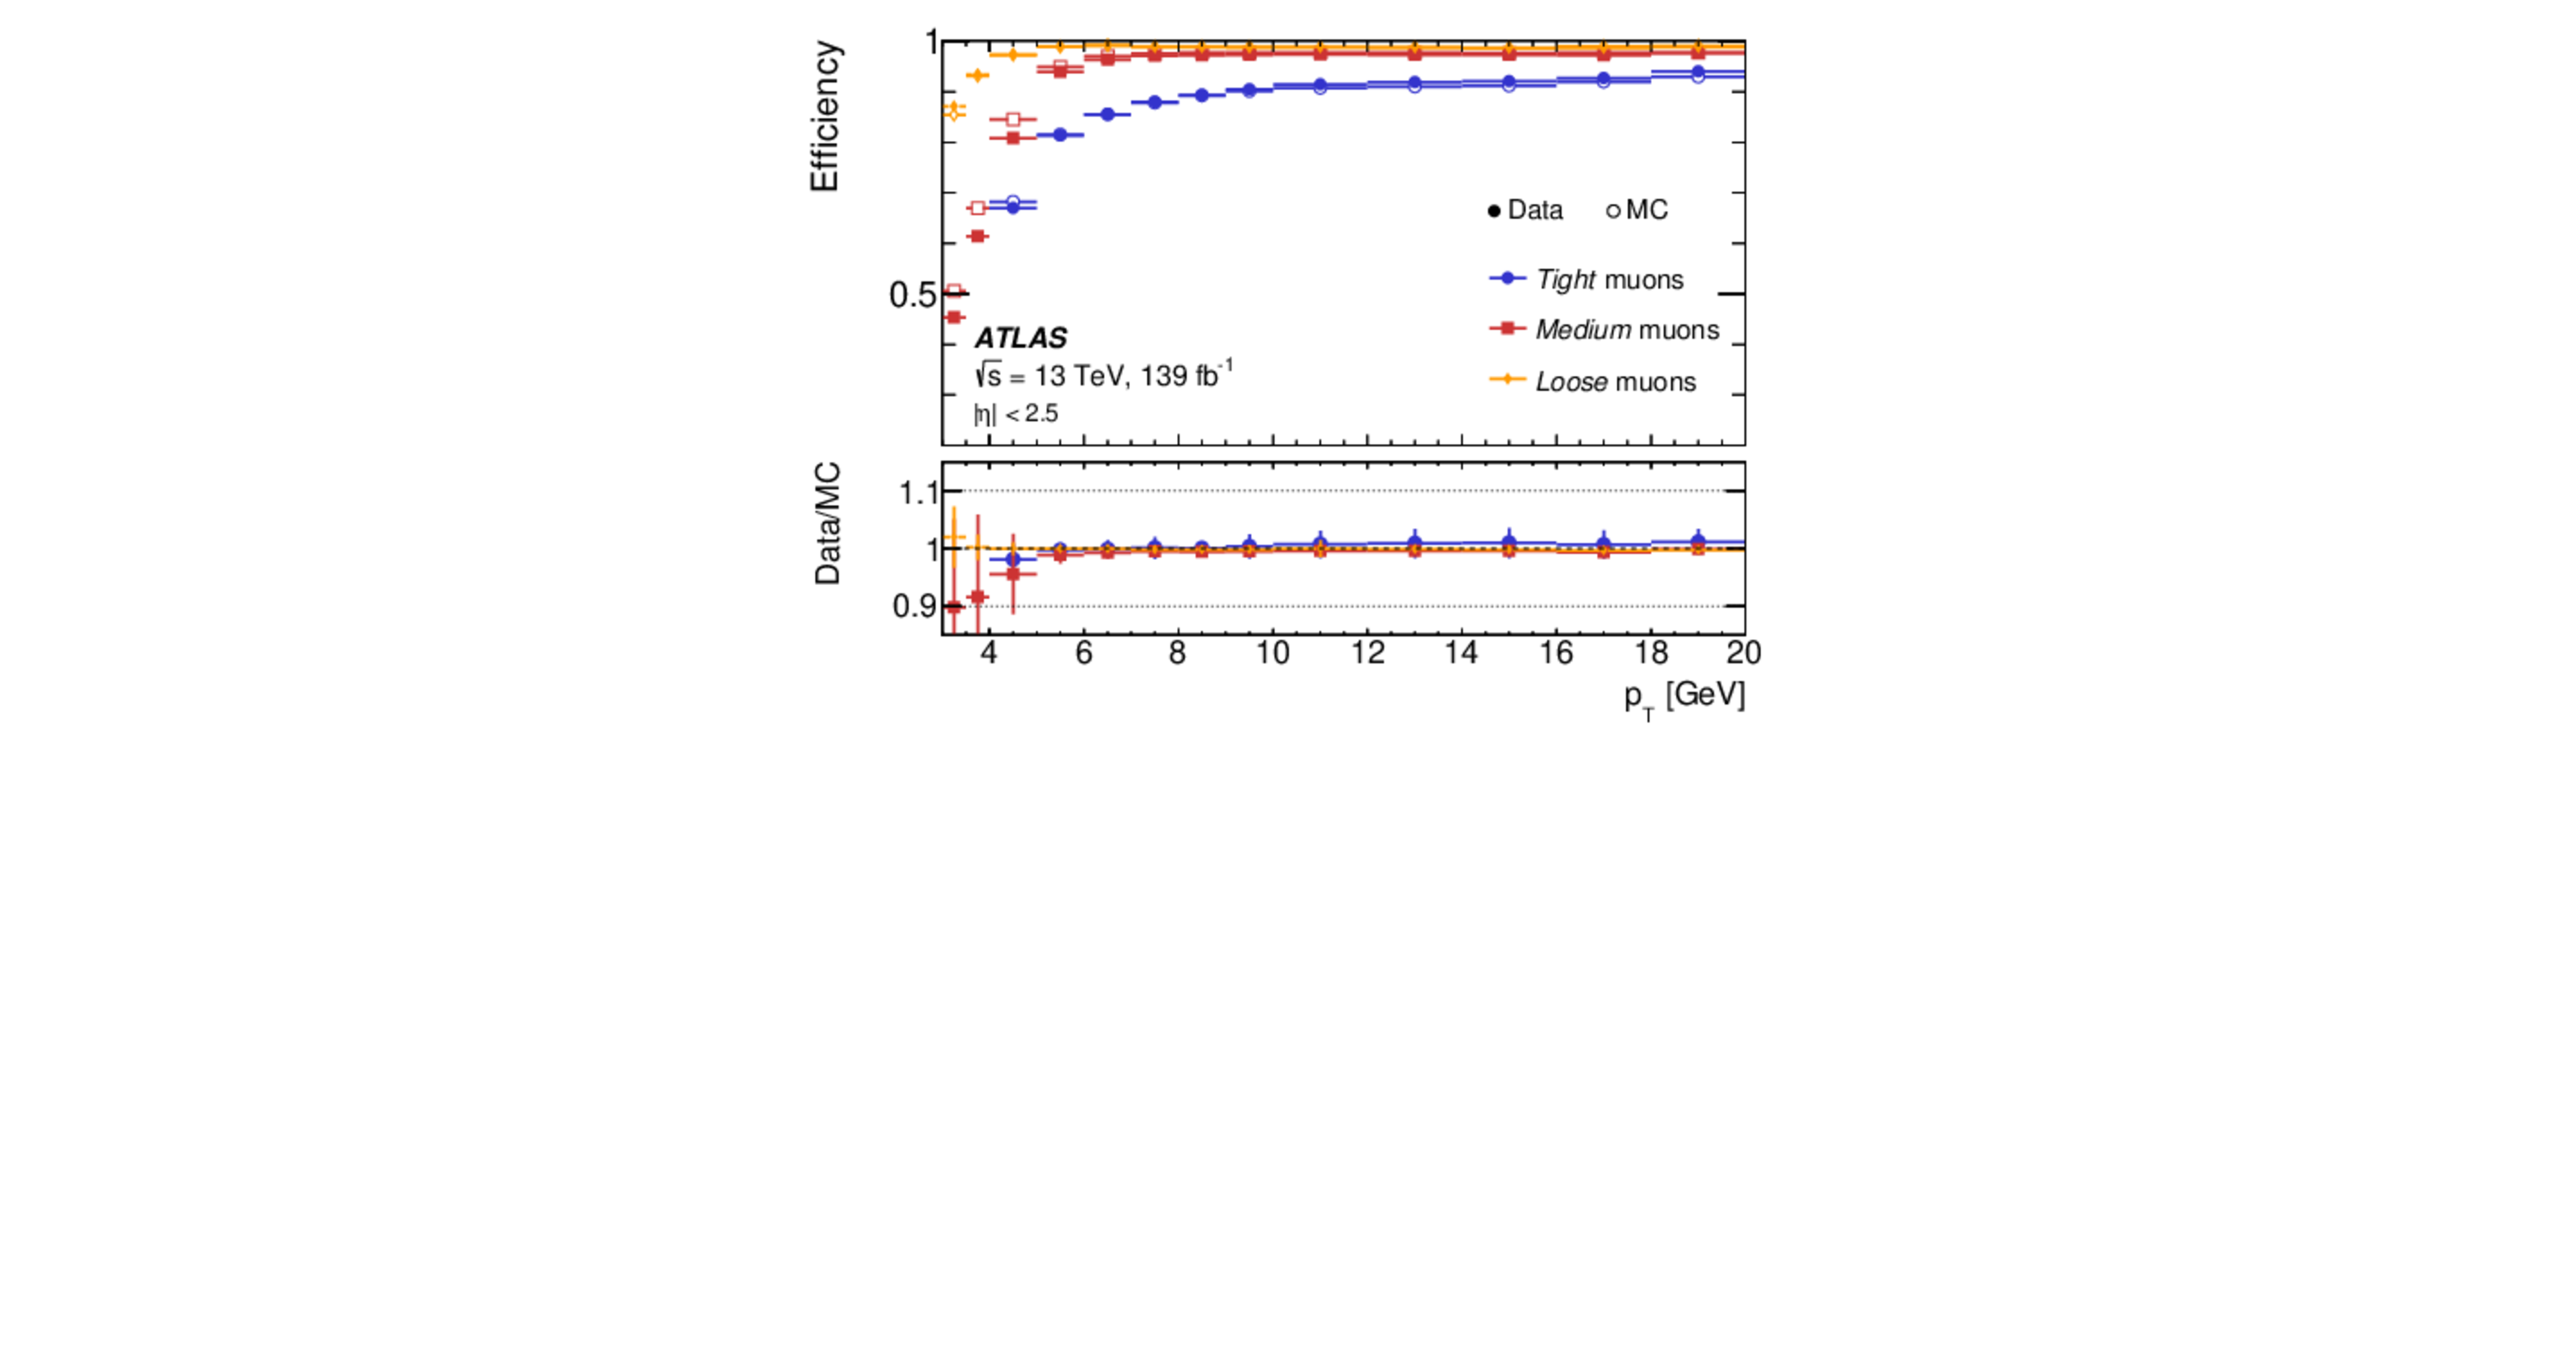
\includegraphics[width=0.45\textwidth,keepaspectratio]{figures/Reconstruction/recoMuonpT}
 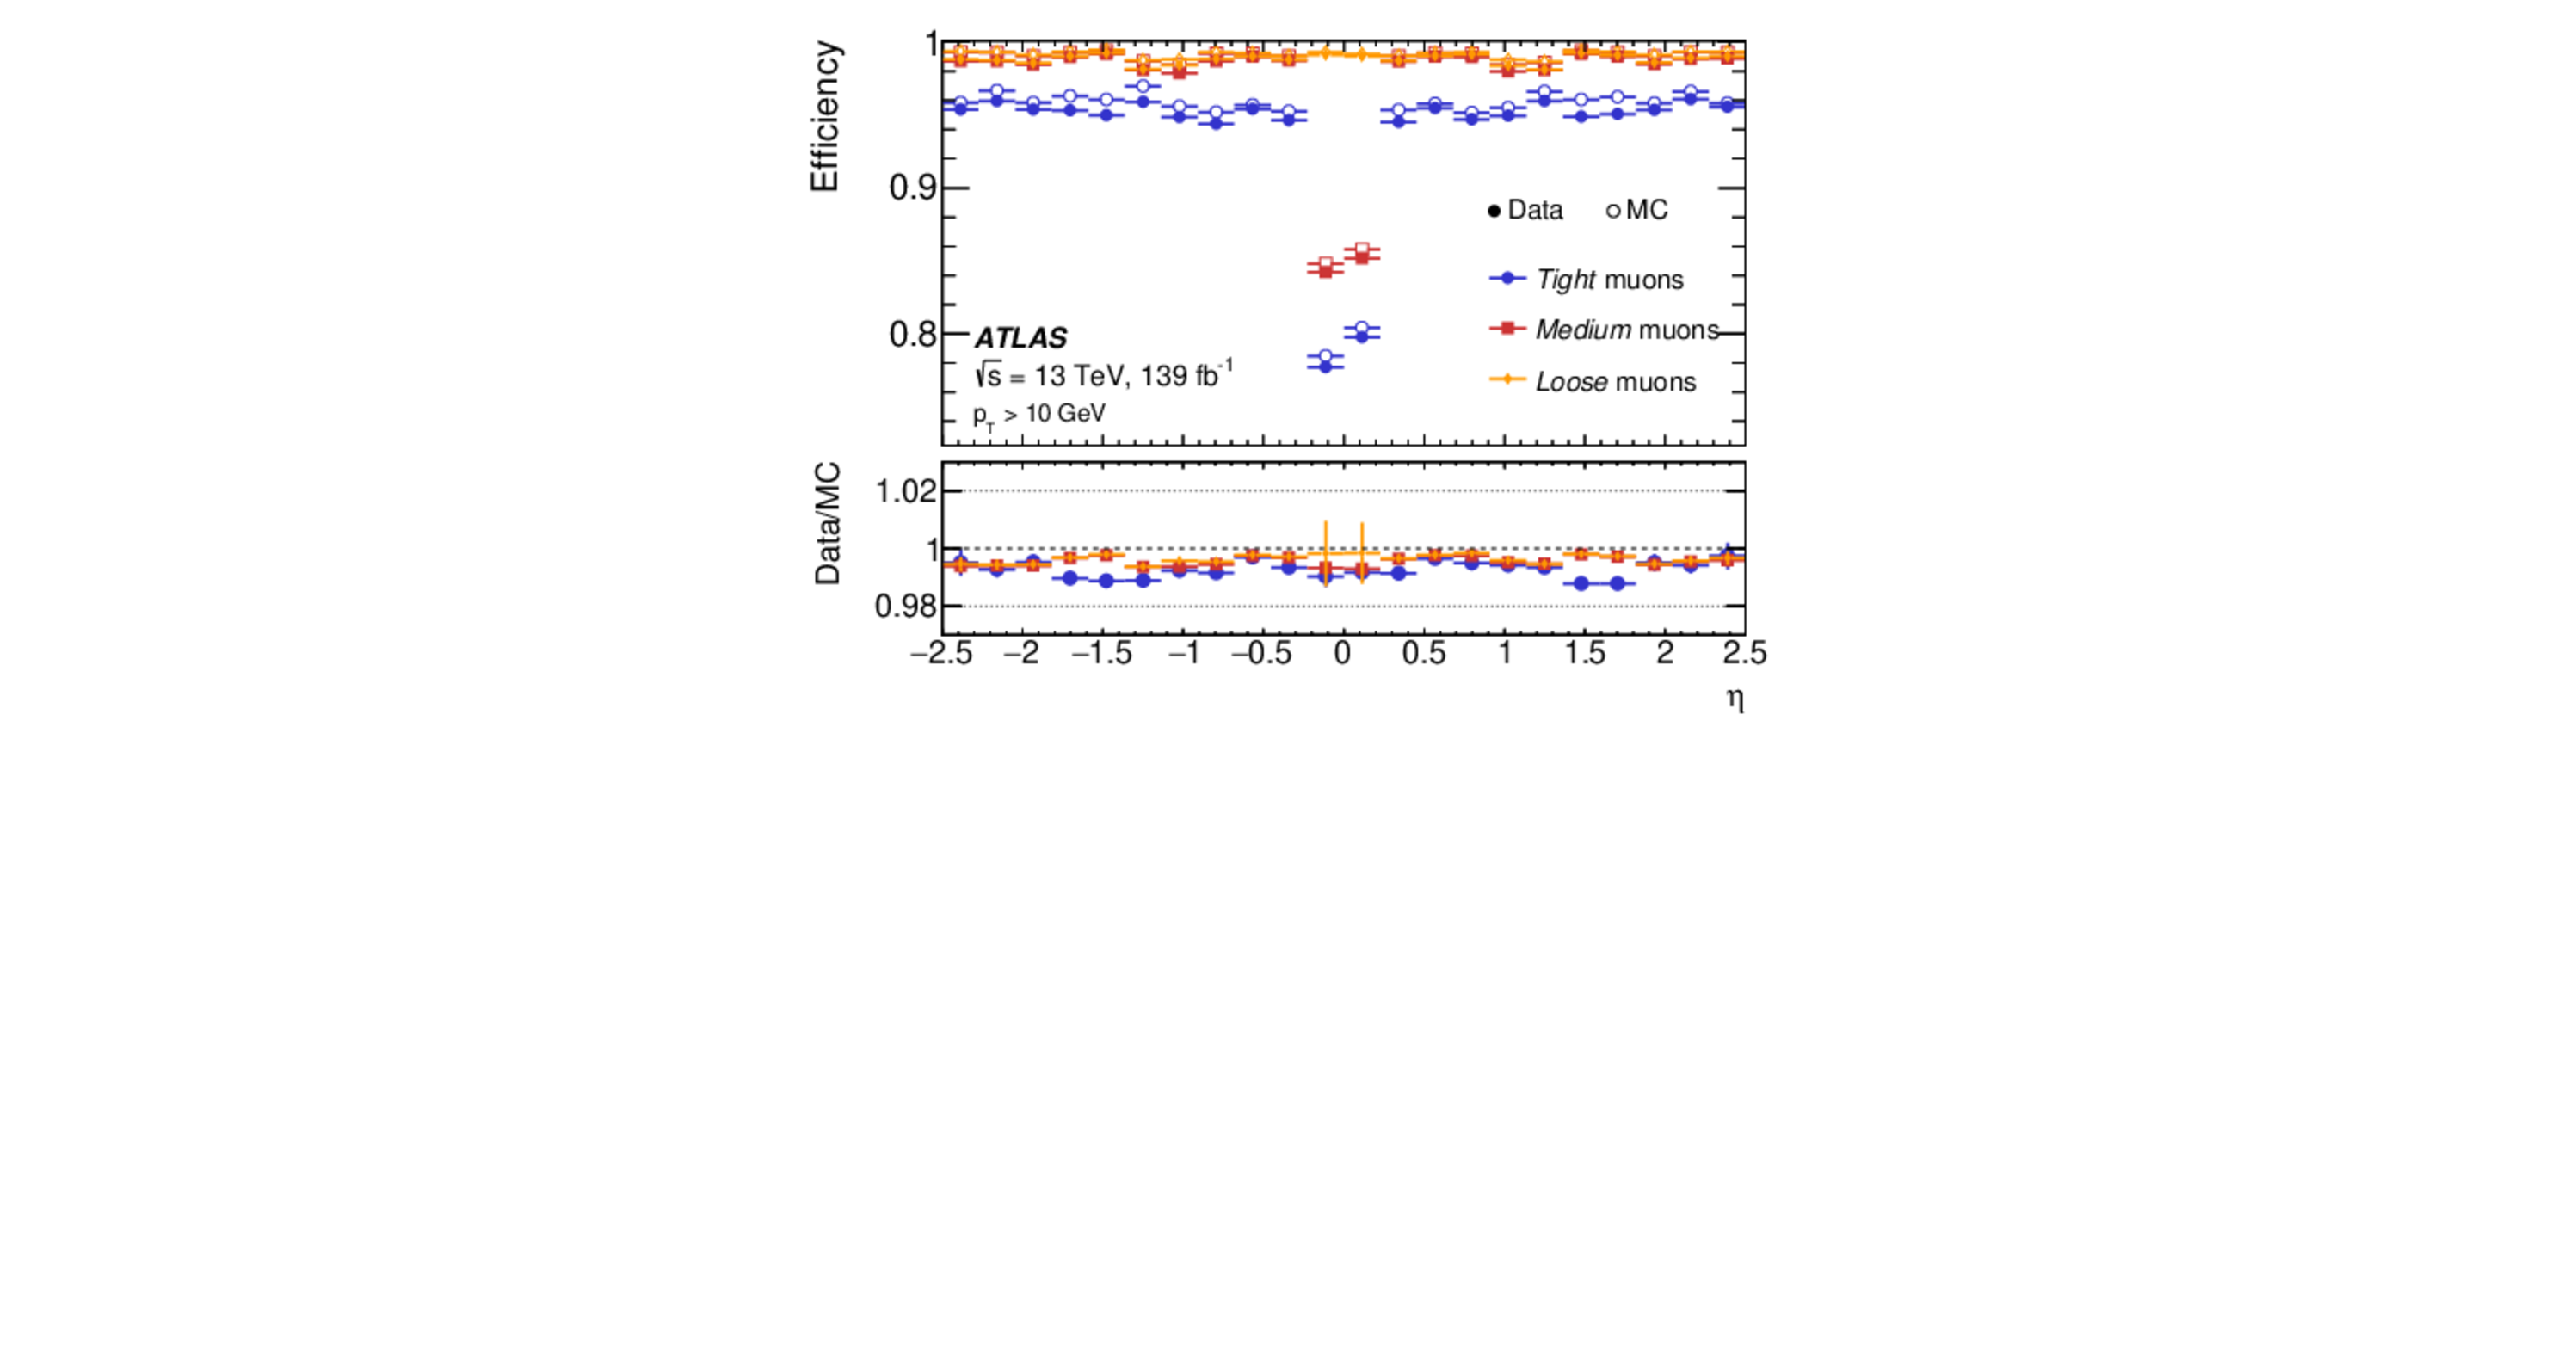
\includegraphics[width=0.45\textwidth,keepaspectratio]{figures/Reconstruction/recoMuonEta}
%}
\caption{
muon reconstructing and identification efficiency with respect to $E_T$ (left) and $eta$ (right) \cite{MUON-2018-03}
}
\label{fig:recoMuon}
\end{center}
\end{figure}
Muon identification is performed by applying quality requirements that suppress background, mainly from pion and kaon decays. 
%It also selects prompt muons with high efficiency and/or guaranteeing a robust momentum measurement. 
For Medium muons, the CB tracks required to have more than three hits in at least two MDT layers exept for |$\eta$|<0.1.
%Specifically, the $q/p$ significance, defined as the absolute value of the difference between the ratio of the charge and momentum of the muons measured in the ID and MS divided by the sum in quadrature can be used for distinguish the muons.It is required to have less than seven for the contamination of the hadrons misidentified as muons.
The Loose identification uses all types of Muons. 
All CB and \textcolor{blue}{ME} muons satisfying the Medium requirements are included. 
The identification used in this analysis is shown in Table~\ref{tab:muon_selection}.
\section{Jets}
Spray of hadrons produced by the hadronization of the final-state partons are called jets.
Kinematics of jets ideally reflects the parton kinematics.
Jets are basically reconstructed by grouping topo clusters by the anti-kt algorithm~\cite{Cacciari_2008}, with a radius of $R = 0.4$ (small-$R$ jets) or $R = 1.0$ (large-R jets). The small-R jet contains most of the radiation from the quark or gluon jets. The large-R jets represents the hadronic decays of the heavy, boosted objects like W, Z bosons where two jets from the quarks overlap.
The anti-$k_t$ algorithm defines a measure of distance $d_{ij}$ between the clusters in the calorimeter,
\begin{equation}
d_{i j}=\min \left\{\frac{1}{k_{\mathrm{T}, i}^{2}}, \frac{1}{k_{\mathrm{T}, j}^{2}}\right\} \times \frac{\left(\Delta R_{i j}\right)^{2}}{R^{2}}
\end{equation}
where $k_{T,i}$ is the transverse momentum of the cluster i and $\Delta R_{i j}=\sqrt{\left(\Delta y_{i j}\right)^{2}+\left(\Delta \phi_{i j}\right)^{2}}$ is the distance between the clusters i and j where y is the rapidity. 
The algorithm searches for the minimum $d_{i j}(k)$ combinations and merges them. 
It iterates that procedure until $d_{i j}(k) = d_{i B}(k)$, cluster i is regarded as a jet and in the end the remaining. 
This procedure is repeated until all clusters are grouped into jets.
Figure~\ref{fig:antikt} shows how the clustering performed for example.
%?
%The small-R jets and the large-R jets are both reconstructed using topo-clusters, while only small-R jets use the track information to give better performance of measuring the energy and the momentum of the jets.
%?
\begin{figure}[tbp]
\begin{center}
%\subfigure[]{
 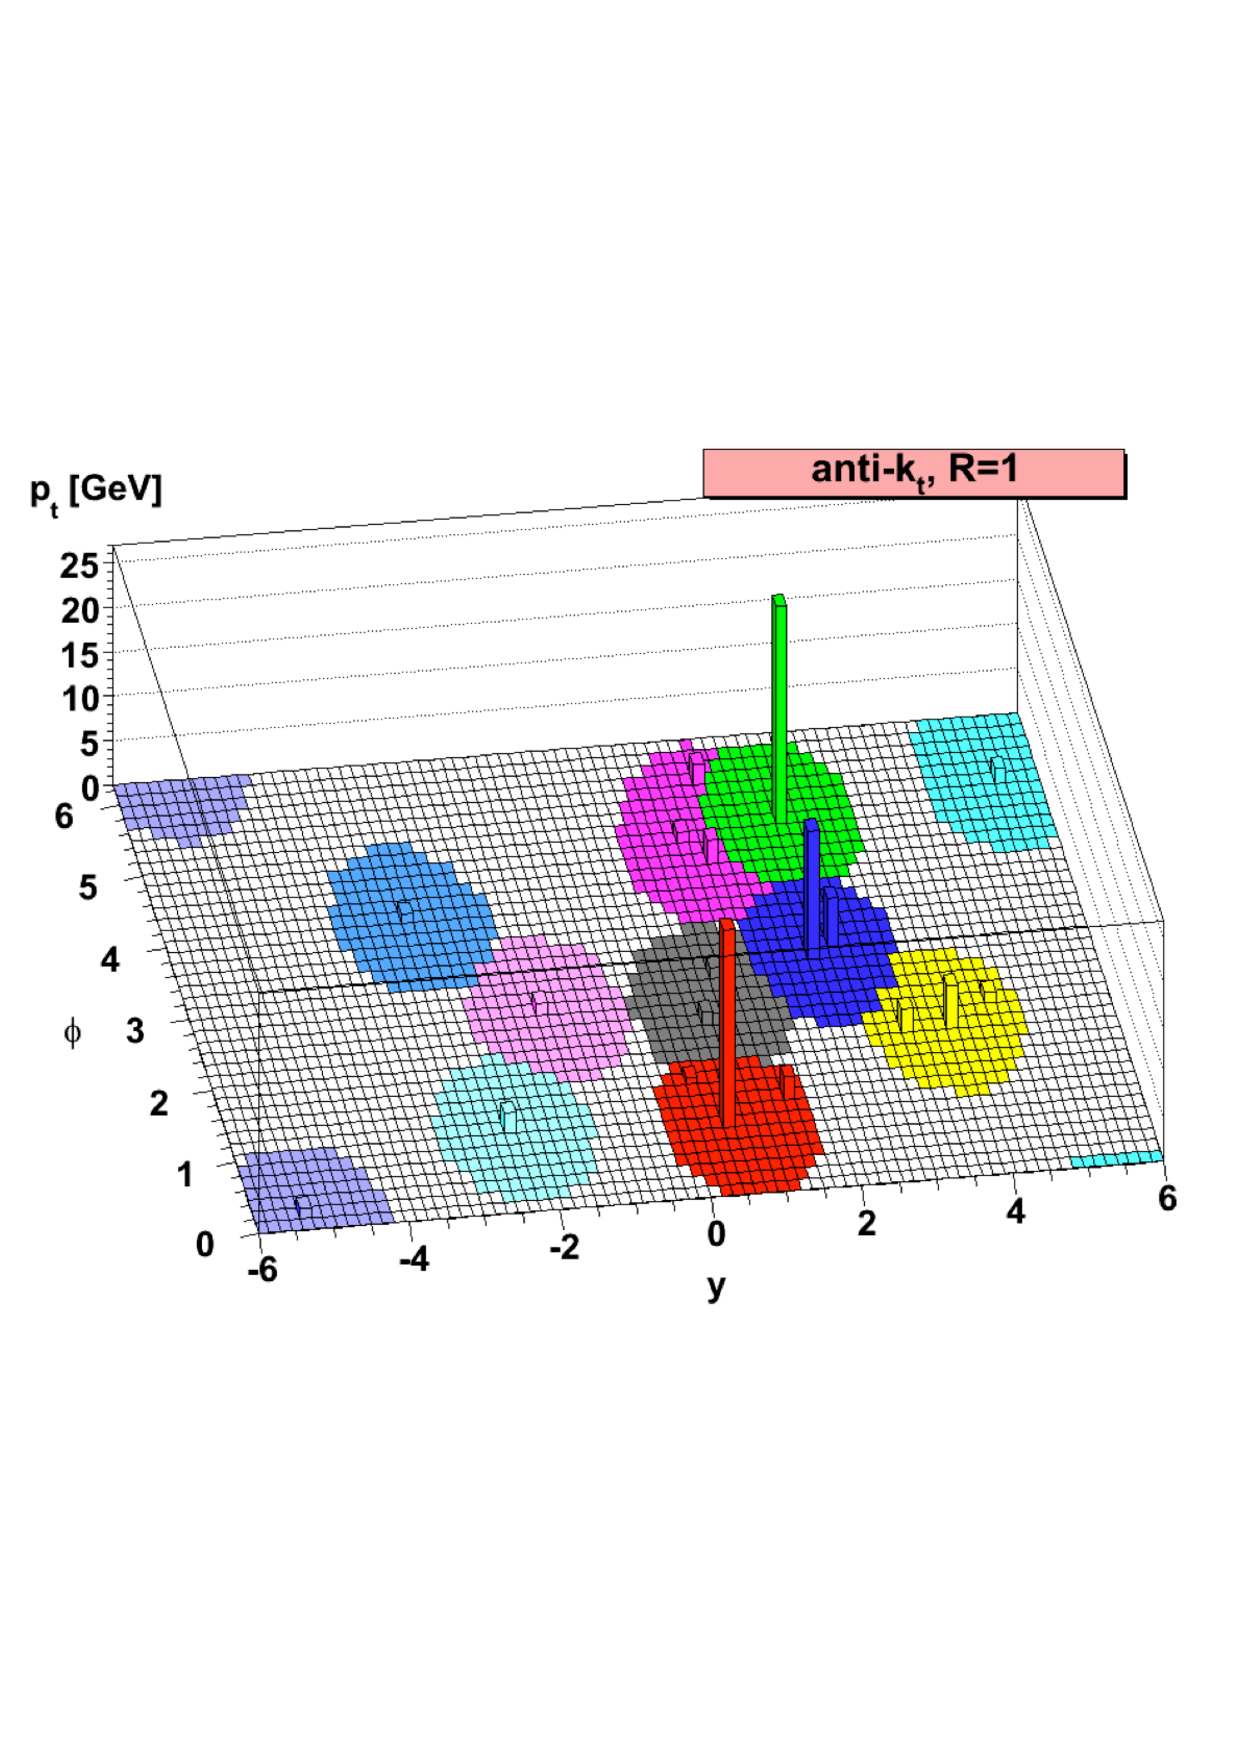
\includegraphics[width=0.70\textwidth,keepaspectratio]{figures/Reconstruction/antikt}
\caption{
anti-$k_T$ algorithm \cite{Cacciari_2008}
}
\label{fig:antikt}
\end{center}
\end{figure}

\subsection{small-R Jets}
The small-R jets are reconstructed using PFlow objets as the input to the anti-$k_T$ algorithm with $R = 0.4$. Particle flow algorithm \cite{PERF-2015-09} is adopted for better measurement of the energy and momentum. The particle flow algorithm uses an ensemble of signals from the calorimeter and the inner tracker. 

The ID tracker information has better resolution for low-$p_T$ particles, and better angular resolution and can trace the particles to hard-scatter
interaction or pile-up. On the other hand, Carolimeters have better resolutions for high $p_T$ and can get neutral particles. Therefore the combined information can improve energy and angular resolution, as well as reduce the pile-up contributions.
%put somewhere the description about pile-ups
In the particle flow algorithm, firstly tracks from the ID are selected, then the tracks to corresponding topo-clusters are matched to them. Secondly energy from the cluster depending on tracks position and $p_T$ is subtracted, and the tracks and remaining topo-clusters constitute the PFlow objects.

%calibration
The calibration for the jets are done with several steps in order to do the correction for all detector effects. 
\begin{itemize}
    \item \textbf{\sf{pileup-substruction}} \\
    The per-event pileup contributions to the $p_T$ of each jets are removed based on each area. It is subtracted based residual $N_{PV}$ and $\mu$ (average interaction per crossing) \cite{JETM-2018-05}.
    The corrected jet $p_T$ is described as:
    \begin{equation}
     p_{T}^{\text {corr }}=p_{T}^{\text {reco }}(-\rho \times A)-\alpha\left(N_{P V}-1\right)-\beta\langle\mu\rangle
    \end{equation}
    This correction with repect to $\eta$ is shown in Figure~\ref{fig:pileup}.
    \begin{figure}[tbp]
    \begin{center}
    %\subfigure[]{
    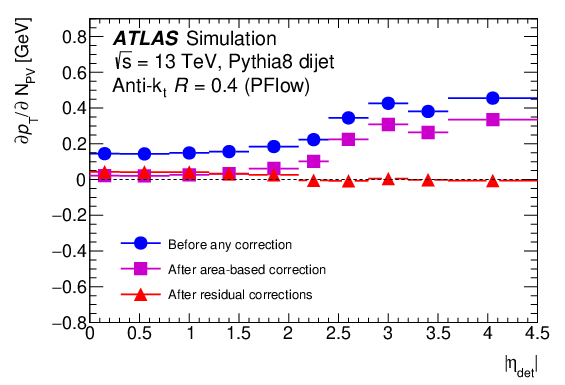
\includegraphics[width=0.45\textwidth,keepaspectratio]{figures/Reconstruction/intimepileup}
    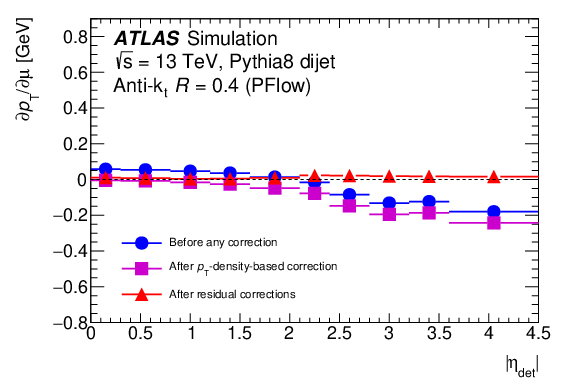
\includegraphics[width=0.45\textwidth,keepaspectratio]{figures/Reconstruction/outtimepileup}
    \caption{
    pile-up subtraction \cite{JETM-2018-05}
    }
    \label{fig:pileup}
    \end{center}
    \end{figure}
    \item \textbf{\sf{MC-based JES, $\eta$, calibration}} \\
    The detector responses are different across detector, especially at the boundaries between calorimeter technology and the granualarities. Some corrections are applied as function of E and $\eta$, by comparing the reconstructed jets to truth jets (energy response, $\mathrm{E}^{\text {reco }} / \mathrm{E}^{\text {truth }}$ ) which derived from the truth MC \cite{JETM-2018-05}.
    Figure~\ref{fig:JES} shows the jet energy response as a function of $\eta$.
    \begin{figure}[tbp]
    \begin{center}
    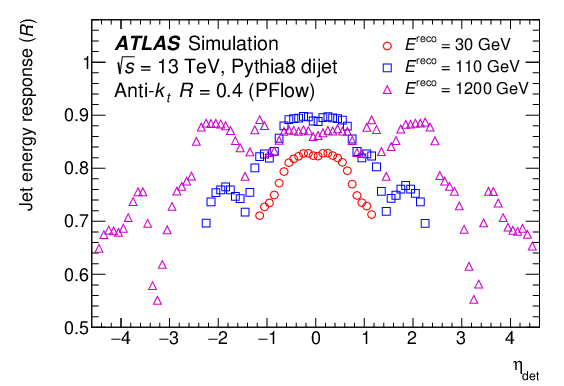
\includegraphics[width=0.60\textwidth,keepaspectratio]{figures/Reconstruction/JES}
    \caption{
    Jet energy response \cite{JETM-2018-05}
    }
    \label{fig:JES}
    \end{center}
    \end{figure}
    \item \textbf{\sf{Global sequential calibration}} \\ 
    The Global Sequential Calibration (GSC) is applied, mainly to accounting for the different response to quark and gluon initiated jets. It also includes the correction for the punch-through, which is jets with large $p_T$ whose energy is not fully contained in calorimeter \cite{JETM-2018-05}.
    \item \textbf{\sf{In-situ validation}} \\
    The last calibration step is a correction with respect to the data. This is a adjustment for potential difference between data and MC, and this is only applied to the data.
    This calibration uses methods which rely on well-calibrated reference objects in the event to constrain the jet $p_T$ response. 
    Sets of the measurements are combined to give a continuous calibration curves of the ratio of the jet response as a function of jet $p_T$, shown in Figure~\ref{fig:in-situcalibration}.
    \begin{figure}[tbp]
    \begin{center}
    %\subfigure[]{
    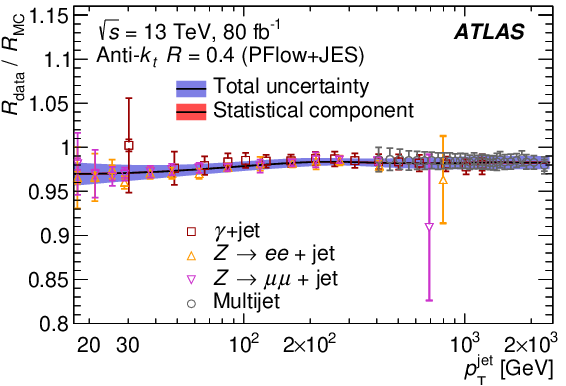
\includegraphics[width=0.6\textwidth,keepaspectratio]{figures/Reconstruction/insitucalibration}
    \caption{
    in-situ calibration \cite{JETM-2018-05}
    }
    \label{fig:in-situcalibration}
    \end{center}
    \end{figure}
\end{itemize}
The total jet energy scale uncertainty with respect to these calibration is shown in Figure~\ref{fig:allJES}.
\begin{figure}[tbp]
    \begin{center}
    %\subfigure[]{
    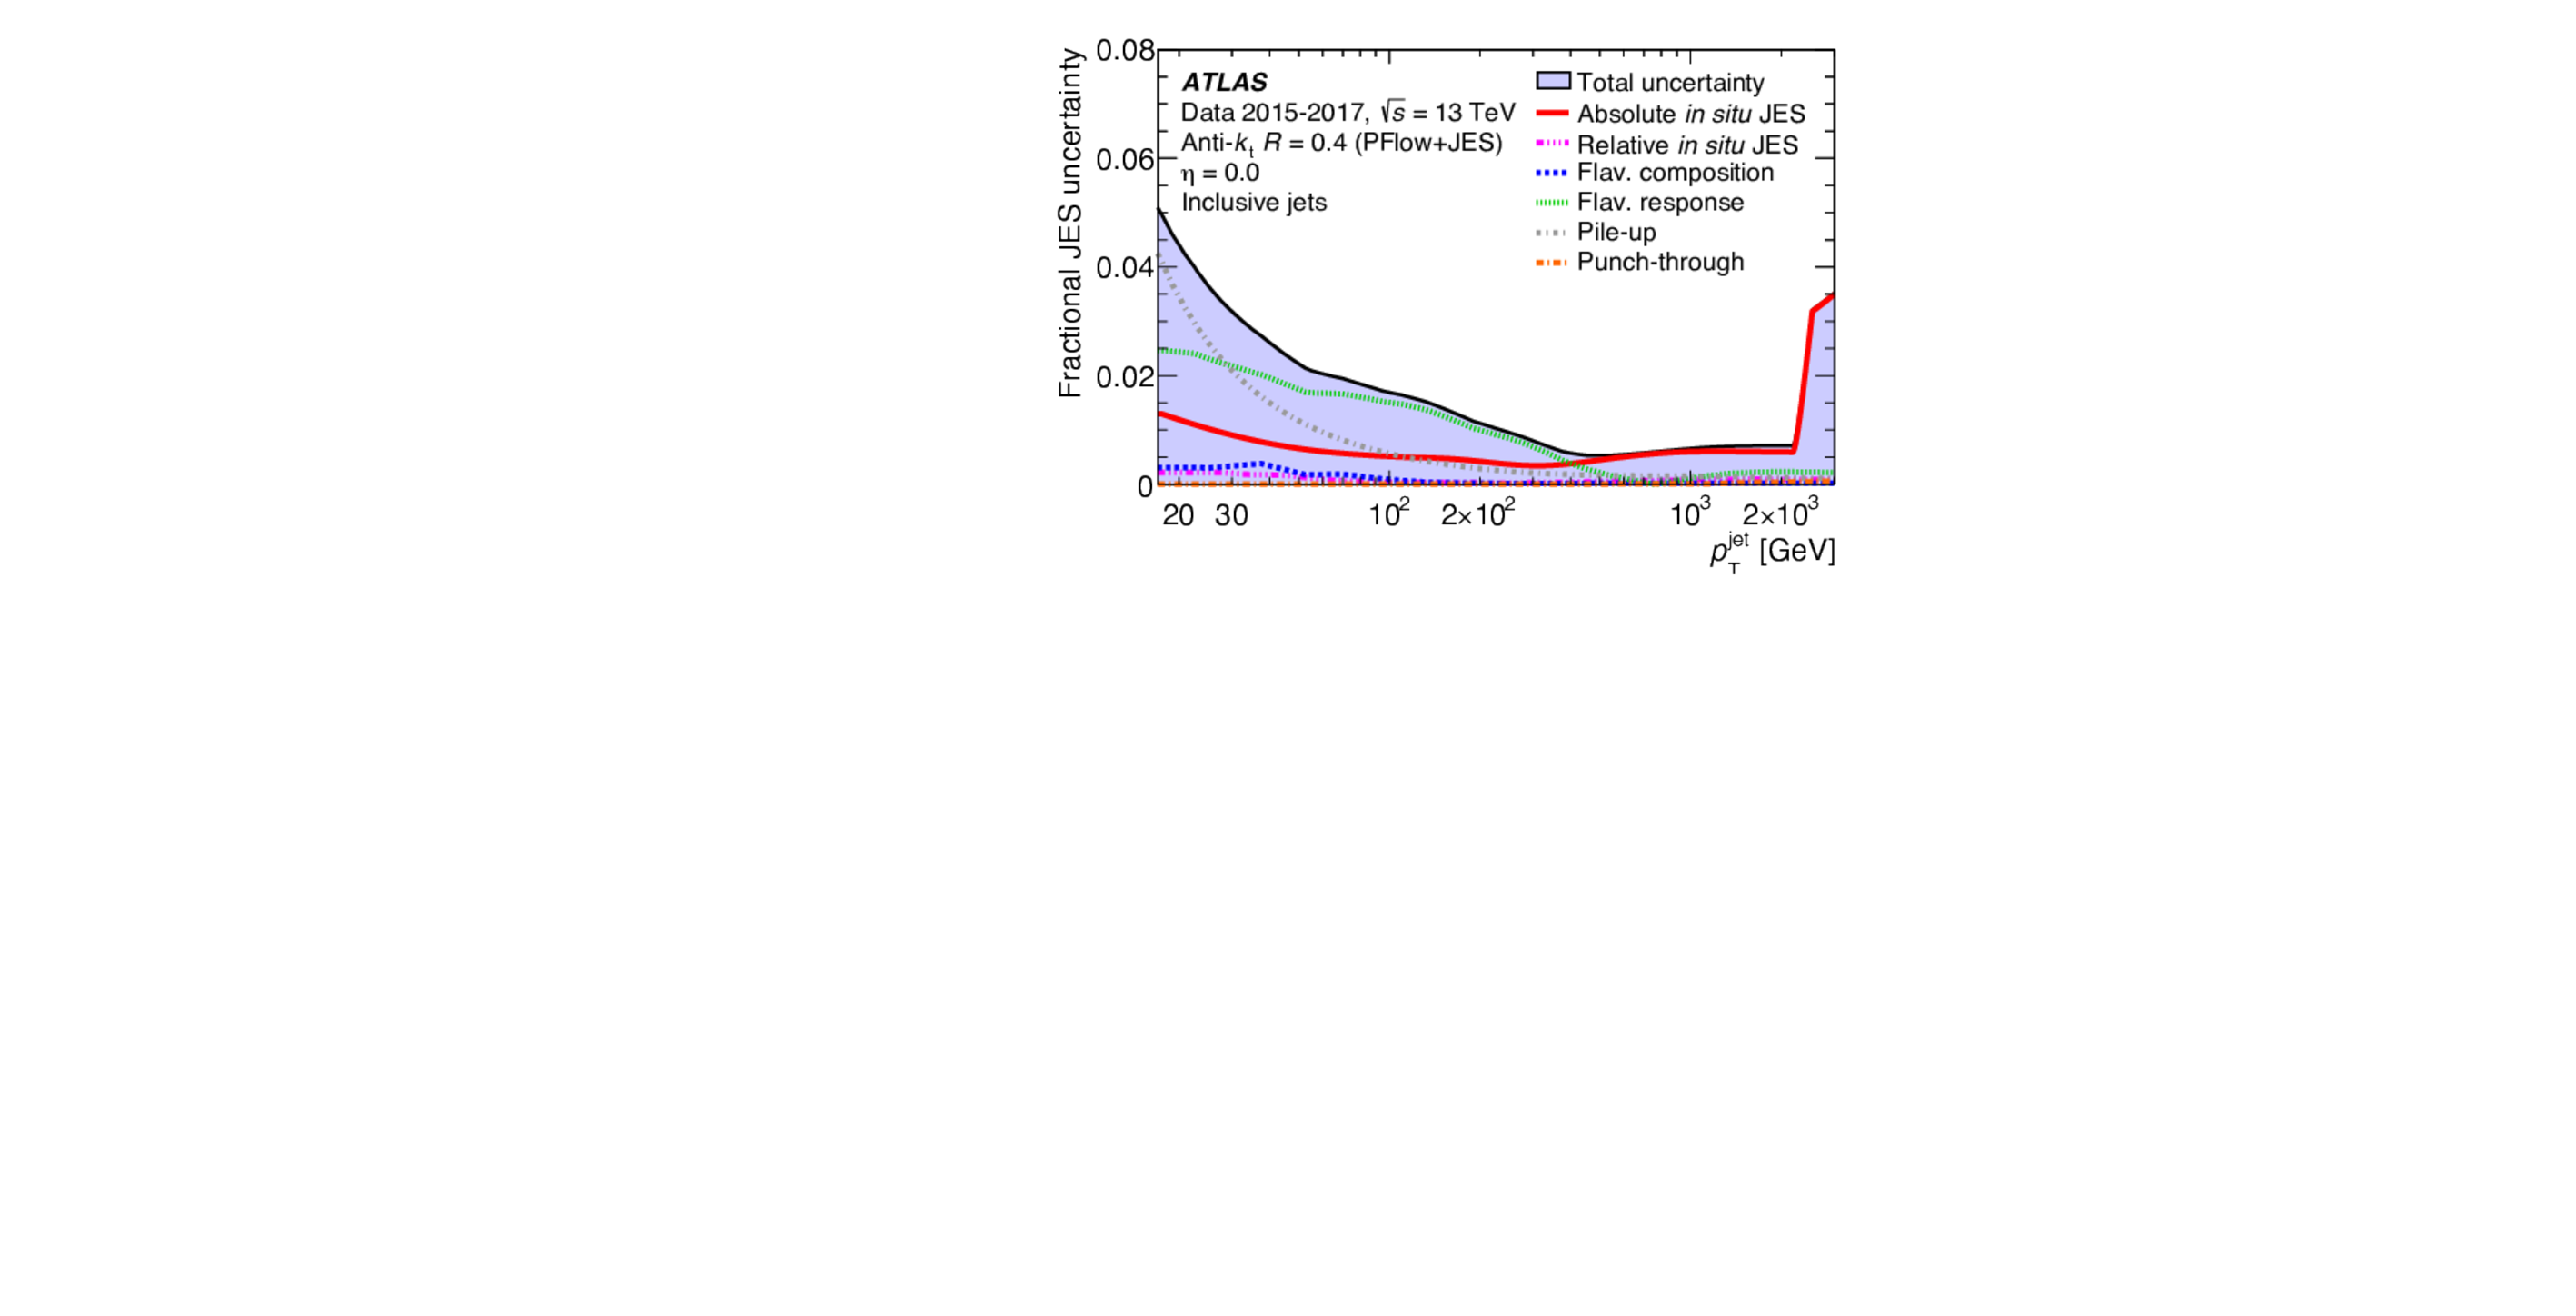
\includegraphics[width=0.6\textwidth,keepaspectratio]{figures/Reconstruction/allJES}
    \caption{
    All JES-related uncertainties is shown in black line. \cite{JETM-2018-05}
    }
    \label{fig:in-situcalibration}
    \end{center}
\end{figure}
%identification

The small-R jets are required to be $p_T$ > 20~GeV ($|\eta|$<2.5) and > 30~GeV (2.5 < $|\eta|$ < 4.5).
The jet vertex tagger (JVT) is applied to identify the jets only from the hard interaction. Furthermore, in the context of the pile-up suppression, forward jet vertex tagger (fJVT) has been introduced, motivated by the forward-like topology in this analysis.
The b-tagging is used for rejecting the jets tagging as including the b-hadrons, to suppress the top contributions.

The identification of small-R jets are summarized into the Table~\ref{}.


\subsubsection{JVT}
\subsubsection{fJVT}

\subsubsection{B-tagging}
The small-R jets containing a b-hadron are identified by DL1r algorithm~\cite{ATL-PHYS-PUB-2020-009}, using a deep-learning neural network.
%The DL1r b-tagging is based on the features of b-hadrons in terms of the impact parameter of tracks and the displaced vertices reconstructed in the inner detector.
The Dl1r combines four low-level tagger, IP3D~\cite{ATL-PHYS-PUB-2017-013}, SV1~\cite{ATL-PHYS-PUB-2017-011}, JetFitter~\cite{ATL-PHYS-PUB-2018-025}, and RNNIP~\cite{ATL-PHYS-PUB-2017-003}.
The so-called b-tagging algorithm is used to distinct b jets from c jets or light jets, which initiated by c-quarks or gluons,u,d,s quarks respectively.
The lifetime of the b hadrons are long enough to travel several mm from the primary interaction before decaying, and create secondary vertices. These can be reconstrcuted using the tracks from the inner detector.
The IP3D uses signed impact parameter significance. The impact parameter, $d_0$ denotes the distance between tracks and the primary vertex as shown in Figure~\ref{fig:bdecay}.
The SV1 reconstructs the secondary vertex in a jets. The JetFitter reconstructs the topology of b/c-hadron decay chains using Kalman filter~\cite{FRUHWIRTH1987444}.
Additionally, the RNNIP uses the track features including the track quality informations.
At last the DL1r combines the outcomes all of these four low-level tagger by deep-learning neural network algorithm.
%The DL1r output and the efficiency of the b-tagging using DL1r are shown in Figure~\ref{}.
In this analysis the b-tagging working point is fixed at 70\% efficiency.

\subsection{large-R Jets}
large-R jets are reconstructed with topo-cluster using anti-$k_T$ algorithm similar to the small-R jets but with R = 1.0. The calibration applied for the large-R jets are mainly same as the procedure with the small-R jets, described in subsection~\ref{}, though there are some specific calibrations for large-R jets.

What is specific to the large-R jet is that the reconstructed topo-clusters are highly contaminated by the calorimeter noises, particles from pile-up, soft radiations. Therefore it is firstly applied grooming and then applied MC and in-situ calibrations. The definition of the jet mass used in the anlysis is combined mass:

\begin{itemize}
    \item \textbf{\sf{Grooming}} \\
    Grooming techniques reduce contributions from pile-up and soft and wide angle emmissions. Trimming algorithm \cite{Krohn2010} is used for this analysis. The original R = 1.0 jet is reclustered into the subjet with R = 0.2, then only subjets with $p_T$ > 5\% of the original jet $p_T$ are remained.
    The detailed calibration is provided for these trimmed jets.
    \item \textbf{\sf{MC-based JES, $\eta$, mass calibration}}\\
    The JES is evaluated as a ratio of their energy to the truth jets as the function of jet energy and $\eta$. The jet mass scale (JMS)  calibration using the jet mass response of reconstrcted jets to the truth is also applied.
    Figure~\ref{fig:largeRresponse} shows the jet energy and mass reponse. 
    \begin{figure}[tbp]
    \begin{center}
    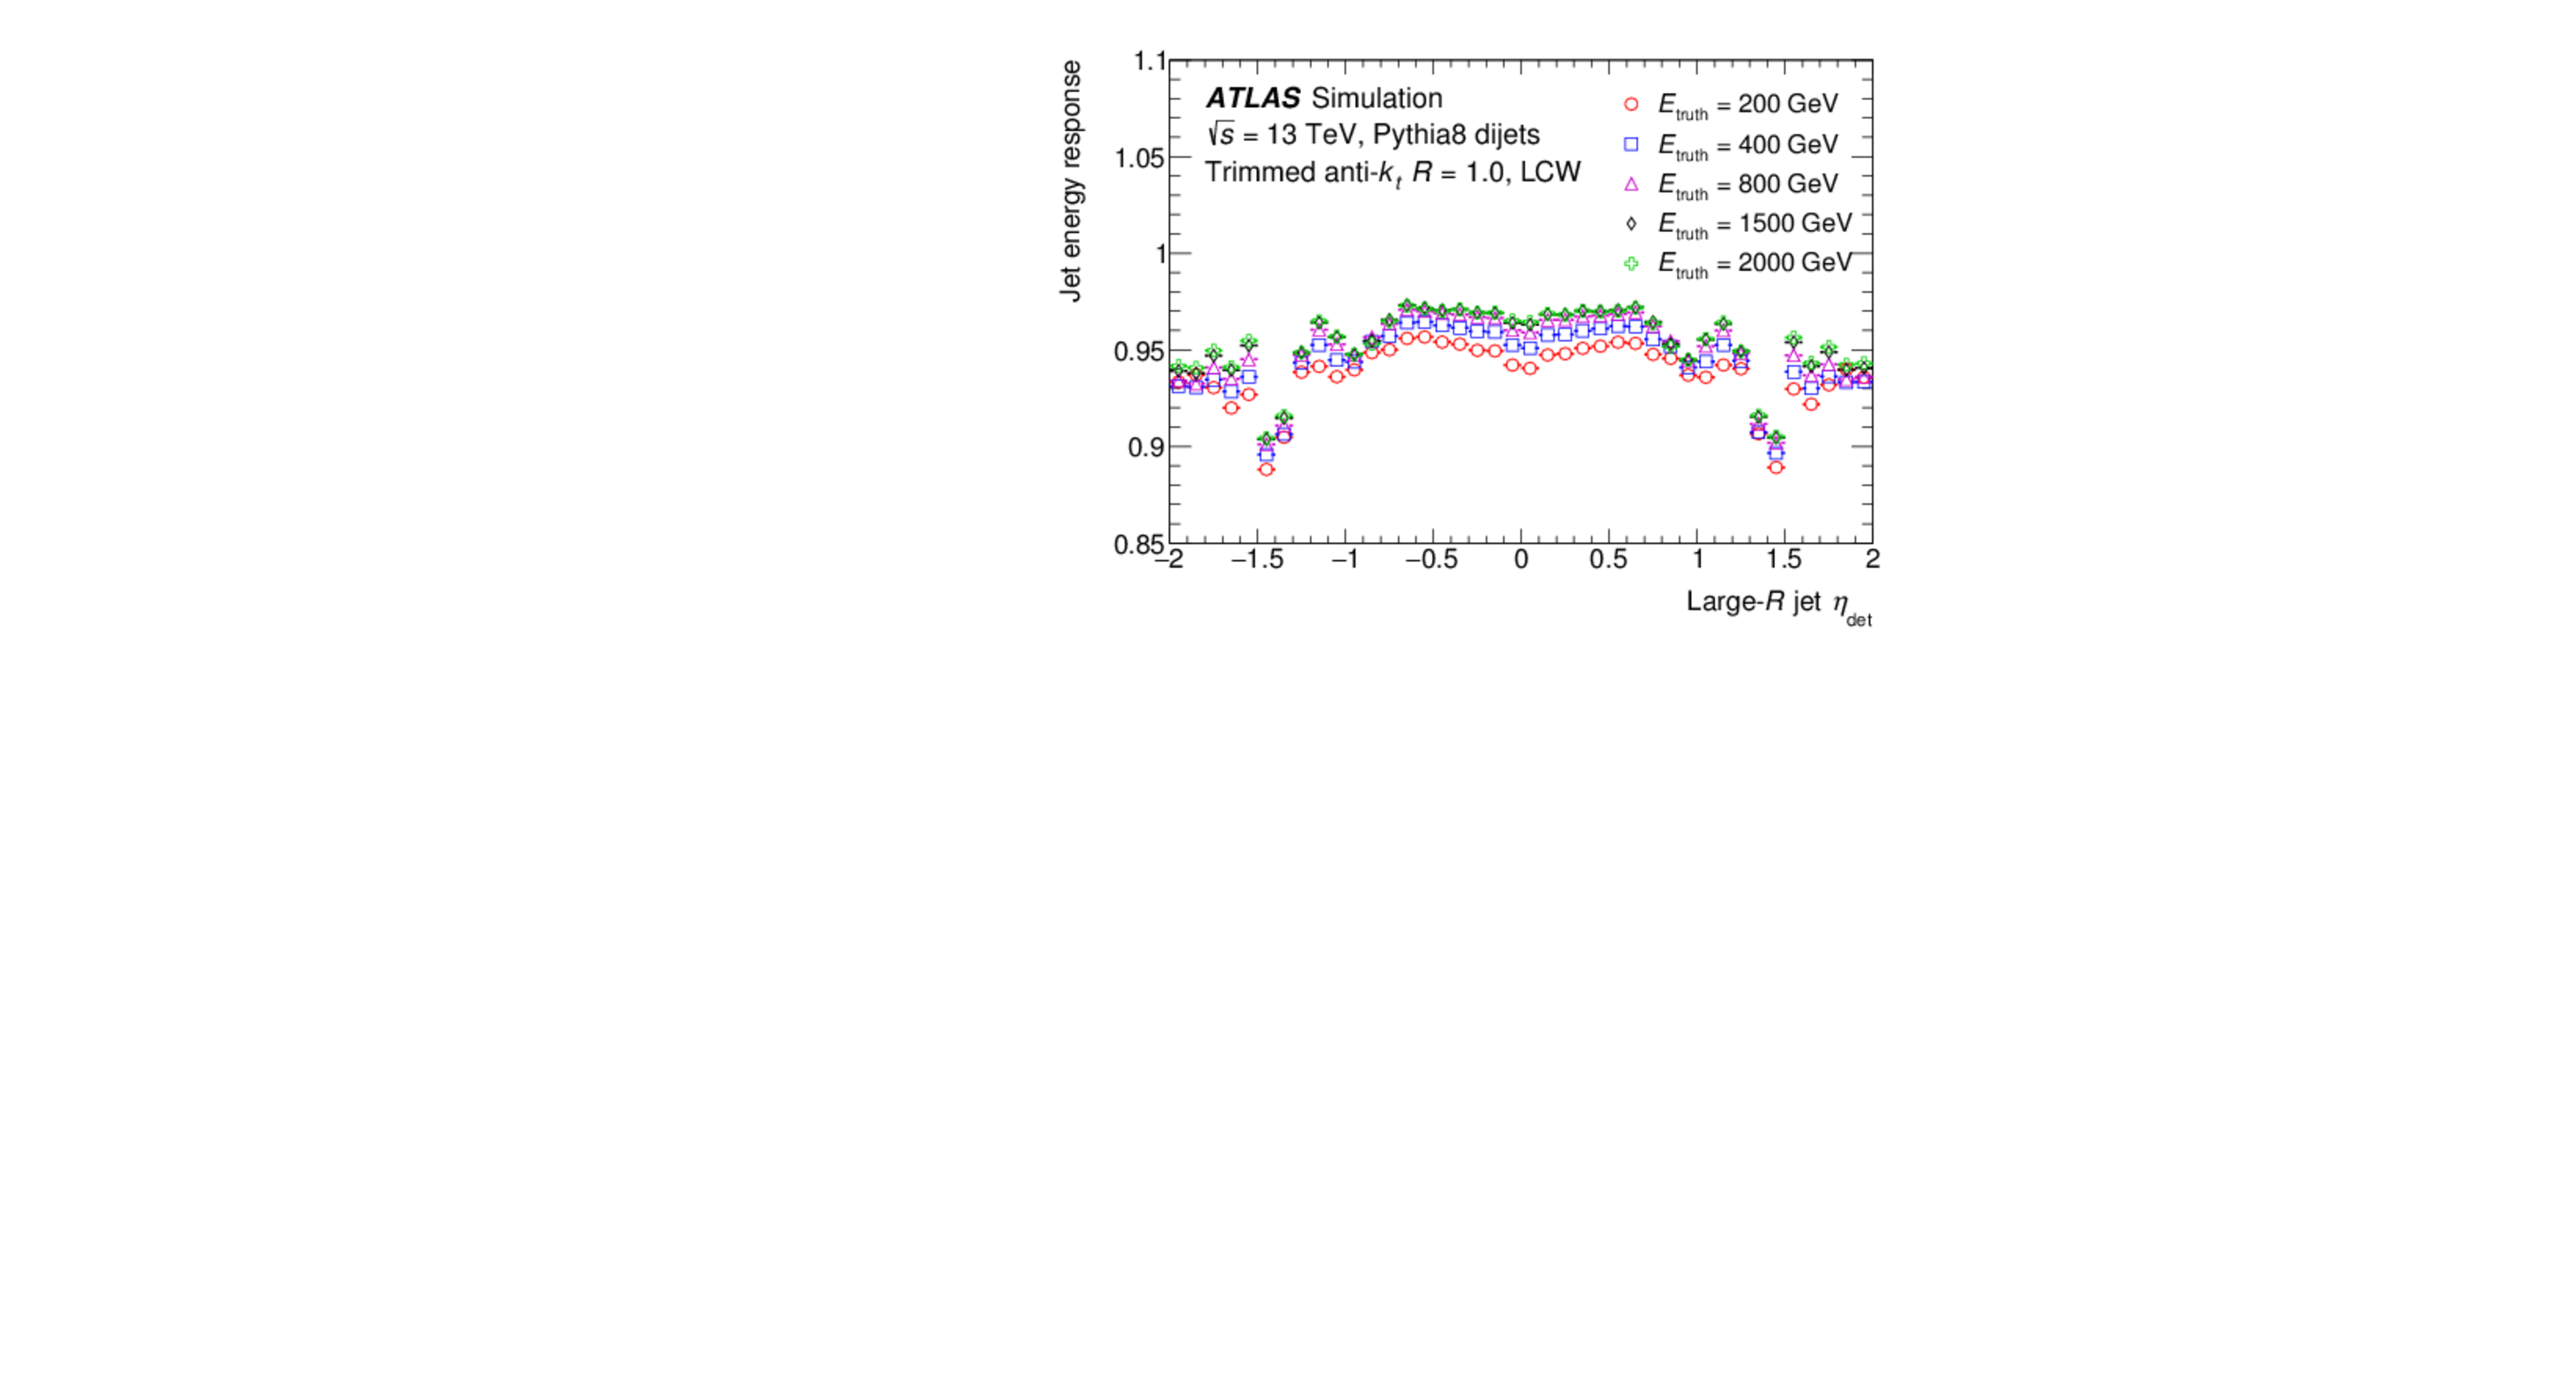
\includegraphics[width=0.45\textwidth,keepaspectratio]{figures/Reconstruction/responsept}
    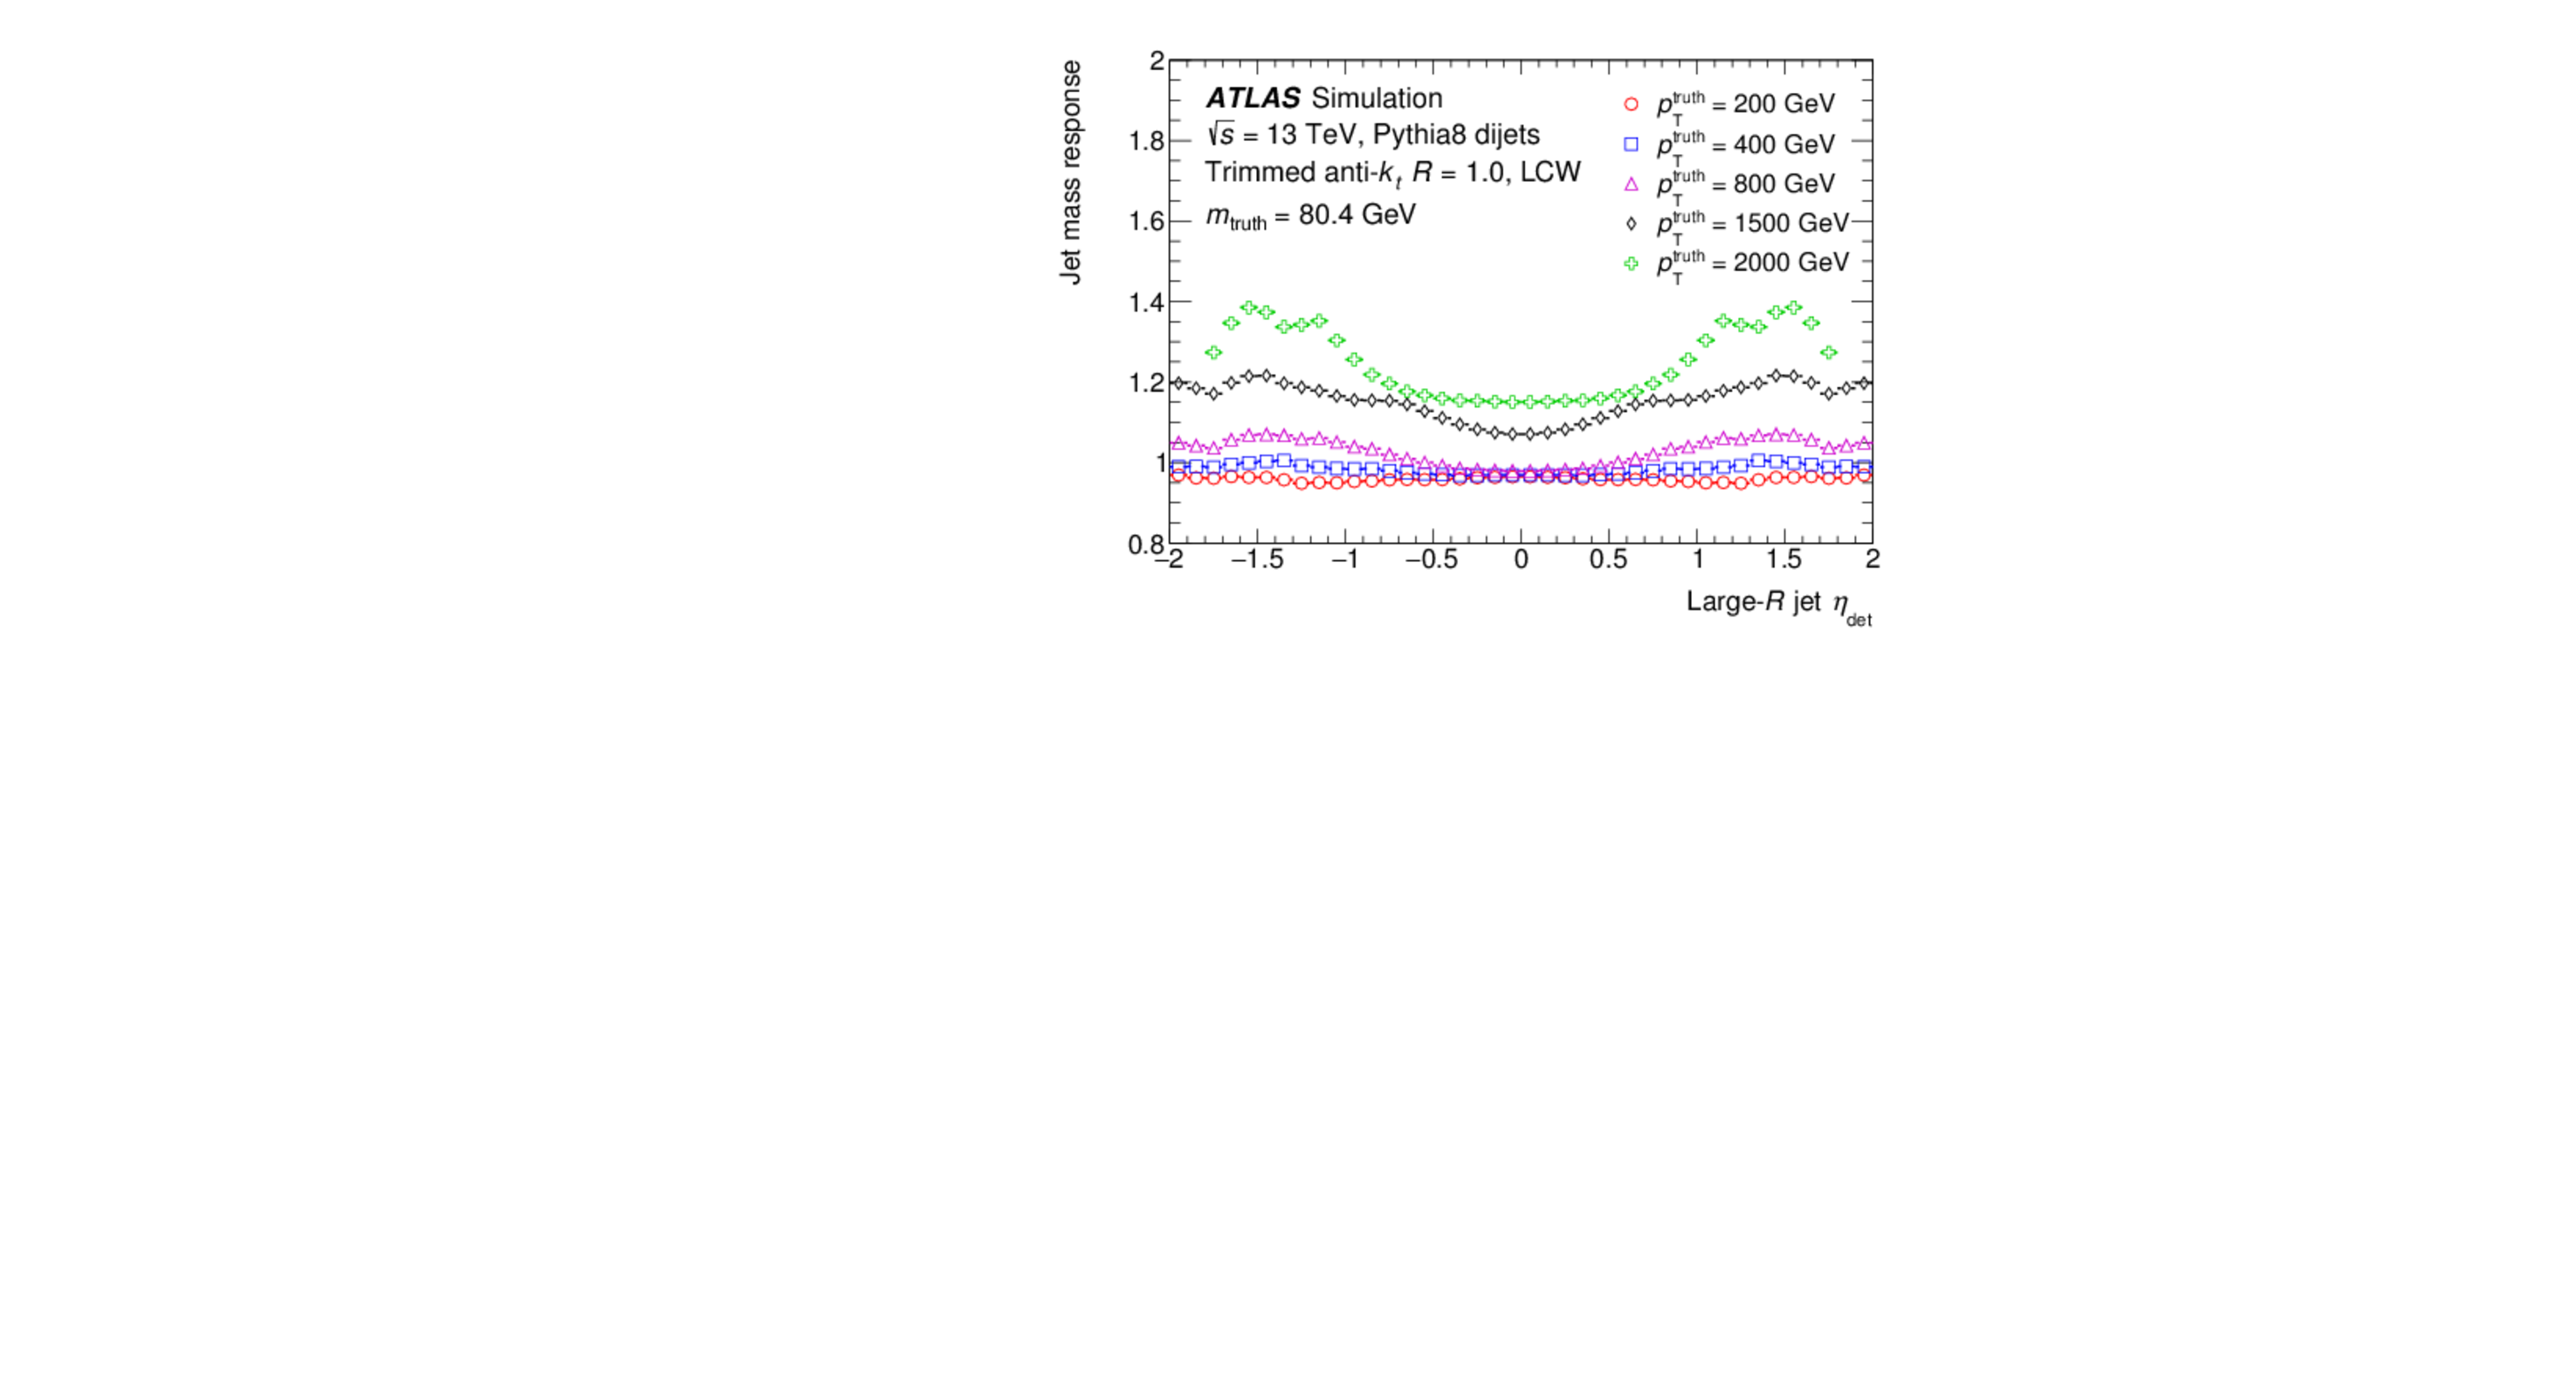
\includegraphics[width=0.45\textwidth,keepaspectratio]{figures/Reconstruction/responsemass}
    \caption{
    jet energy response of large-R jets \cite{JETM-2018-02}
    }
    \label{fig:largeRresponse}
    \end{center}
    \end{figure} 
    \item  \textbf{\sf{In-situ JES and JMS calibration}} \\
    In-situ calibration is applied for the remaining difference of the jet energy between the data and MC. It is performed with similar procedure with small-R jets. The JES is calibrated in events where the jet recoils against a reference object, which are calibrated photon, reconstructed Z boson, or a system of well-measured small-R jets. \cite{JETM-2018-02}. 
\end{itemize}

\subsection{jet substructure}
The large-R jet from boson has 2-prong structure, since it was originally collimated two quarks. This substructure can be the key to distinguish the boson jets to quark or gluon jets, which have 1-prong structure.
Figure~\ref{fig:jetsub} shows the schematic view of the substructure.
 \begin{figure}[tbp]
    \begin{center}
    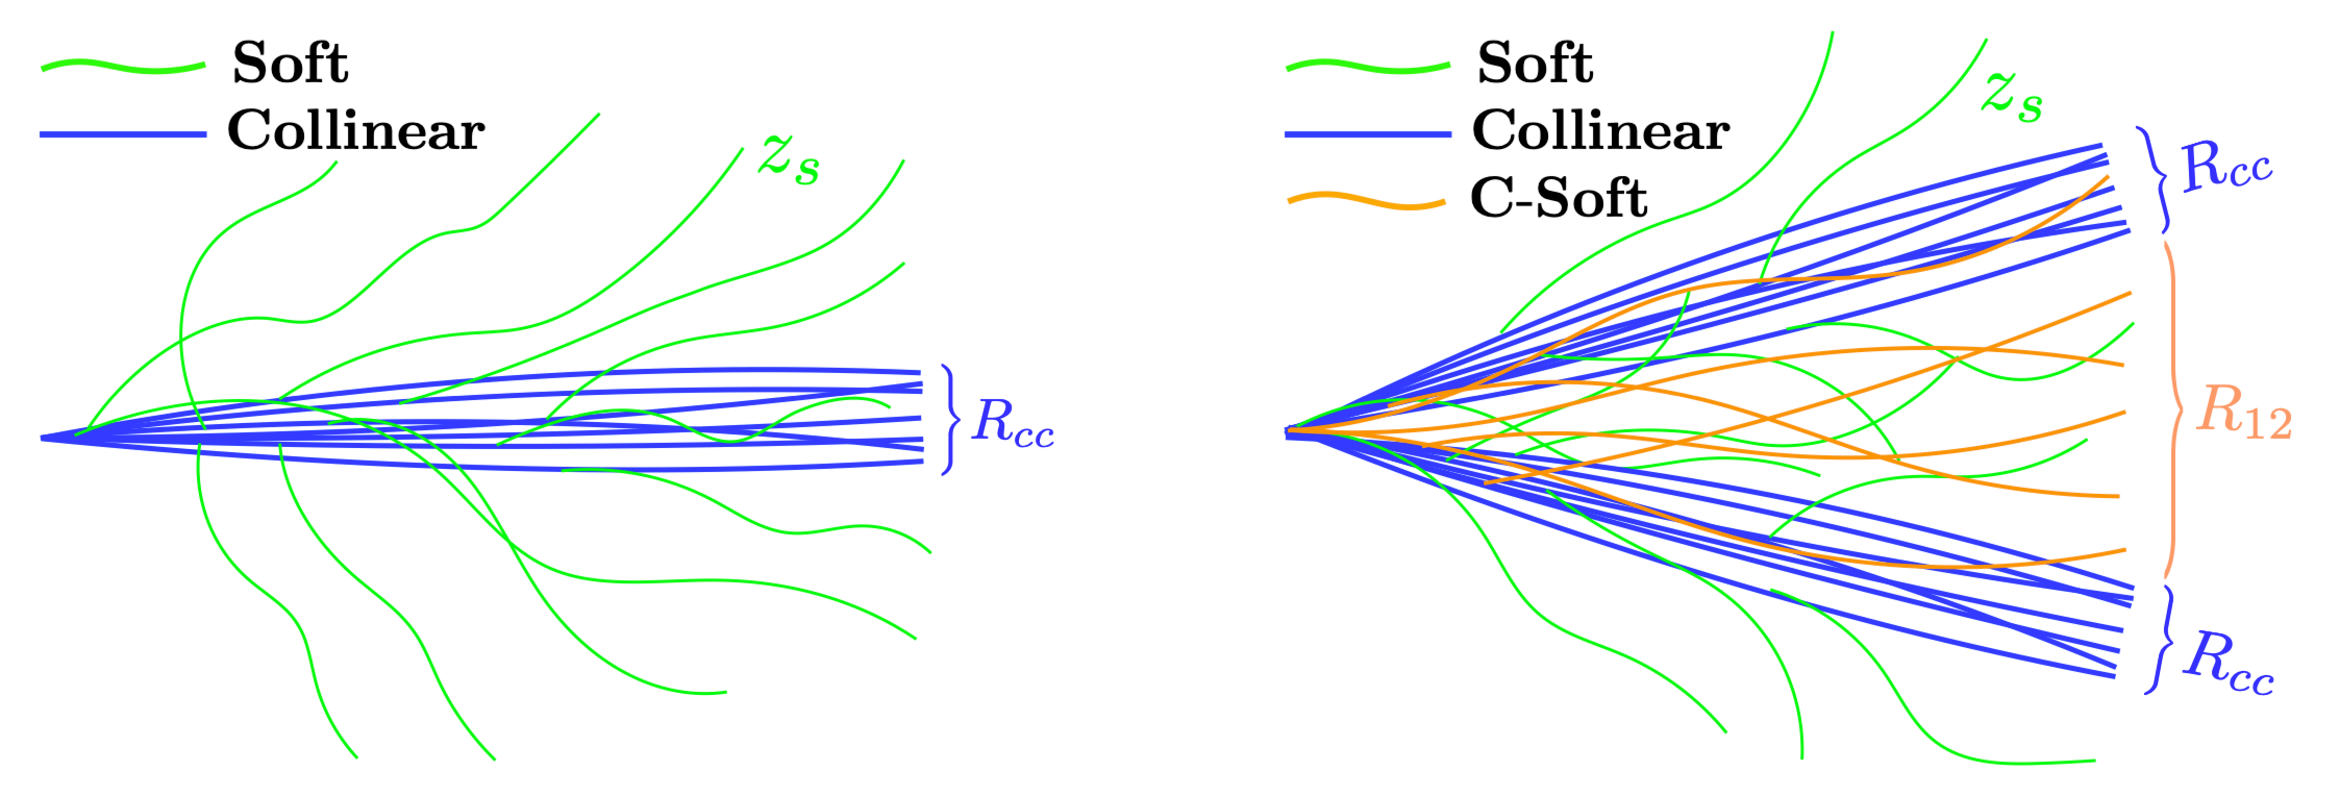
\includegraphics[width=0.80\textwidth,keepaspectratio]{figures/Reconstruction/jetsub}
    \caption{
    jet substructure \cite{Larkoski_2014}
    }
    \label{fig:jetsub}
    \end{center}
    \end{figure}
The jet substructure variable, $D_2$ is used to characterize the structure.  $D_2$ is defined as:
\begin{equation}
D_{2}^{(\beta)}=\frac{e_{3}^{(\beta)}}{\left(e_{2}^{(\beta)}\right)^{3}}
\end{equation}
where the 2 and 3-point energy correlation function $e_{n}^{(\beta)}$ is defined as:
\begin{equation}
\begin{aligned}
e_{2}^{(\beta)} &=\frac{1}{p_{T J}^{2}} \sum_{1 \leq i<j \leq n_{J}} p_{T i} p_{T j} R_{i j}^{\beta} \\
e_{3}^{(\beta)} &=\frac{1}{p_{T J}^{3}} \sum_{1 \leq i<j<k \leq n_{J}} p_{T i} p_{T j} p_{T k} R_{i j}^{\beta} R_{i k}^{\beta} R_{j k}^{\beta}
\end{aligned}
\end{equation}
where $p_{T J}$ is the transverse momentum of the jet with respect to the beam, $p_{T i}$ is the transverse momentum of particle $i$, and $n_{J}$ is the number of particles in the jet. 
The boost-invariant angle $R_{ij}^{2}=\left(\phi_{i}-\phi_{j}\right)^{2}+\left(y_{i}-y_{j}\right)^{2}$ is the distance in the azimuthrapidity plane and for infrared and collinear (IRC) safety, the angular exponent $\beta>0$. 
These energy correlation depends on how the soft and the collinear jet contributions are. The 1-prong and the 2-prong jets can be distinguished by the relation of two function, $e_{3}^{\beta=1} \sim\left(e_{2}^{\beta=1}\right)^{3}$ as shown in Figure~\ref{fig:phasespace23} \cite{Larkoski_2014}. 
\begin{figure}[tbp]
    \begin{center}
    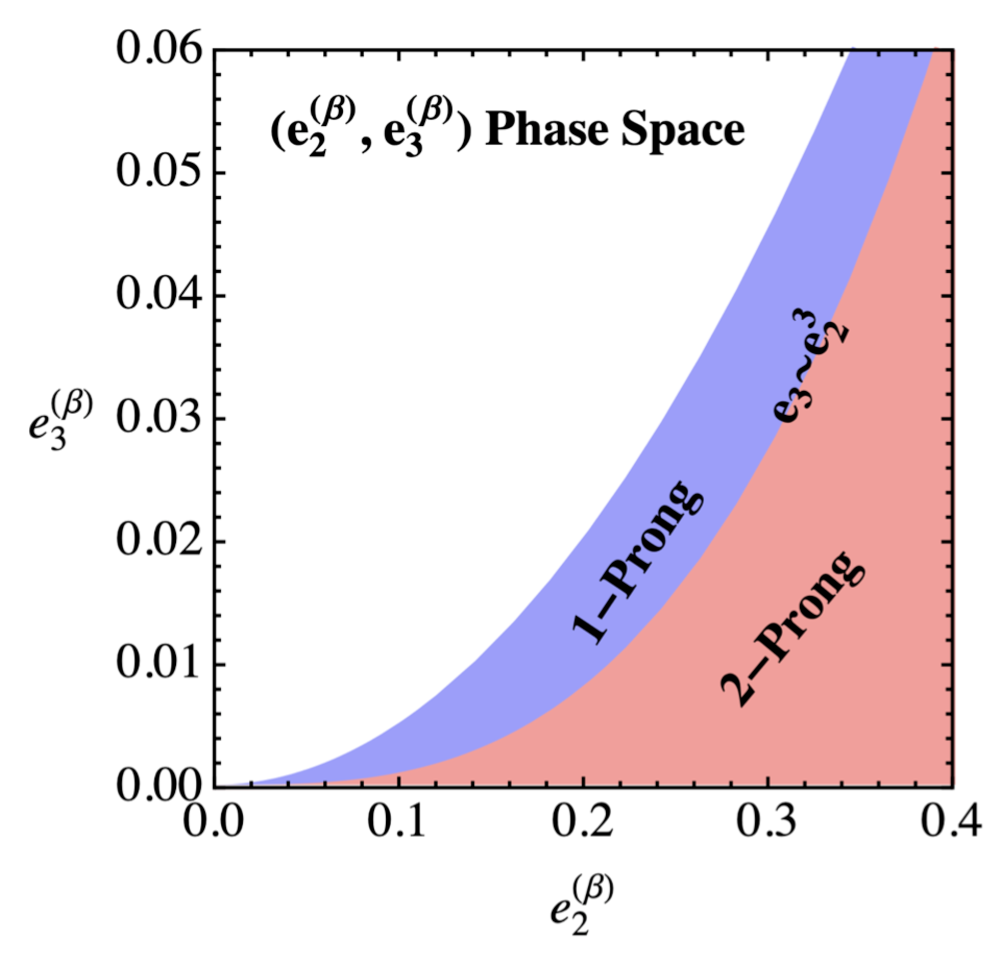
\includegraphics[width=0.50\textwidth,keepaspectratio]{figures/Reconstruction/phasespace23}
    \caption{
    boundaries of energy correlation function \cite{Larkoski_2014}
    }
    \label{fig:phasespace23}
    \end{center}
\end{figure}
The $D_2$ variable tends to get the lower value for 2-prong jet, boson jet while it tends to get the higher value for 1-prong jet, which is q/g jet.
\subsection{Boosted Boson Tagger}
The 3-variable cut-based tagger, that relies on $D_2$, jet mass, and the number of the tracks~\cite{ATL-PHYS-PUB-2020-017} is used for identifying the large-R jet from W/Z boson and to reject the other SM background processes. It provides two fixed working points defined at 50\% and 80 \% signal efficiency. 
large-R jets are required to be $p_T$ > 200~GeV and $|\eta| <2.0$, and jet mass > 50~GeV.
\section{Missing Transverse Momentum}
The particle such as neutrinos traverses the whole detector and cannot be detected in the detector, as the Figure~\ref{fig:ParticlePath} shows. Those invisible particles are reconstructed by using the imbalance of the transverse momenta. It is calculated by taking the negative sum of the momenta of detected objects, electrons, muons, and jets and additionally, so called soft terms, which are charged-particle tracks not matched to the reconstructed objects\cite{PERF-2016-07}.
\section{Overlap Removal}
\textcolor{blue}{Write about overlap removal here}

\section{Triggers}
\textcolor{blue}{Write about the data takings and the triggers here}


